%%%%%%%%%%%%%%%%%%%%%%%%%%%%%%%%%%%%%%%%%%%%%%%%%%%%%%%%%%%%%%%%%%%%%%%%%%%%%%
%%%%%%%%%%%%%%%%%%%%%%%%%%%%%%%%%%%%%%%%%%%%%%%%%%%%%%%%%%%%%%%%%%%%%%%%%%%%%%
%%%%%%%%%%%%%%%%%%%%%%%%%%%%%%%%%%%%%%%%%%%%%%%%%%%%%%%%%%%%%%%%%%%%%%%%%%%%%%

\chapter{Approximating functions} \label{approx:chapter}

%%%%%%%%%%%%%%%%%%%%%%%%%%%%%%%%%%%%%%%%%%%%%%%%%%%%%%%%%%%%%%%%%%%%%%%%%%%%%%

\section{Complex numbers}
\label{sec:complexnums}

\sectionnotes{half a lecture}

In this chapter we look at some of the sequences and series of functions
we already saw and extend the results to a somewhat more general setting,
and we will look at some completely new results.
In particular, we consider complex-valued functions.
We gave complex numbers as examples before, but
let us start from scratch and properly define the complex number field.

A complex number is just a pair $(x,y) \in \R^2$ on which we define
multiplication (see below).
We call the set the complex numbers and denote it by $\C$.
We identify $x \in \R$ with $(x,0) \in \C$.
The $x$-axis is then called the \emph{\myindex{real axis}} and the $y$-axis is
called the \emph{\myindex{imaginary axis}}.  The set $\C$ is sometimes called the
\emph{\myindex{complex plane}}.

Define
\begin{align*}
& (x,y) + (s,t) := (x+s,y+t) \\
& (x,y) (s,t) := (xs-yt,xt+ys)
\end{align*}
Under the identification above we have $0 = (0,0)$ and $1 = (1,0)$.  These
properties then give a field (exercise).

Generally, we write a complex number $(x,y)$ as $x+iy$, where we
define\footnote{Note that engineers use $j$ instead of $i$.}
\begin{equation*}
i := (0,1) .
\end{equation*}
Notice that $i^2 = (0,1)(0,1) = (0-1,0+0) = -1$.
So we have a solution to the polynomial equation
\begin{equation*}
z^2+1=0 .
\end{equation*}
From now on, we will not use the notation $(x,y)$ and use only $x+iy$.
See \figureref{fig:complexplane}.
\begin{myfigureht}
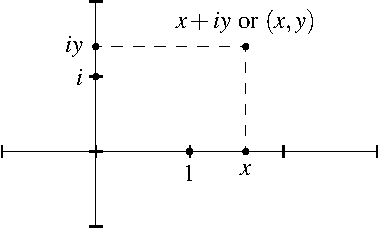
\includegraphics{figures/complexplane}
\caption{The points $1$, $i$, $x$, $iy$, and $x+iy$ in the complex
plane.\label{fig:complexplane}}
\end{myfigureht}

We generally use $x,y,r,s,t$ for real values and $z,w,\xi,\zeta$
for complex values, although that is not a hard and fast rule.  In
particular $z$ is often just used as a third real variable in $\R^3$.

\begin{defn}
Let $z= x+iy$.
Define
the \emph{\myindex{real part}} of $z$ as $x$, and the
the \emph{\myindex{imaginary part}} of $z$ as $y$.  We write
\begin{equation*}
\Re\, z := x , \qquad
\Im\, z := y .
\end{equation*}
Define the
\emph{\myindex{complex conjugate}} as
\begin{equation*}
\widebar{z} := x-iy .
\end{equation*}
Similarly define \emph{\myindex{modulus}} as
\begin{equation*}
\sabs{z} := \sqrt{x^2+y^2} .
\end{equation*}
\end{defn}
The modulus acts like an absolute value.  For example,
$\sabs{zw} = \sabs{z} \, \sabs{w}$ (exercise).

Think of the complex conjugate as a reflection across the real axis.
We note that the real numbers are precisely those for which the imaginary
part $y=0$.  In particular they are precisely those numbers which satisfy
the equation
\begin{equation*}
z = \widebar{z} .
\end{equation*}

As $\C$ is really $\R^2$, we let the metric on $\C$ be the standard
euclidean metric on $\R^2$.
In particular,
\begin{equation*}
\sabs{z} = d(z,0) , \qquad 
\text{and also} \qquad 
\sabs{z-w} = d(z,w) .
\end{equation*}
So the topology on $\C$ is
the same exact topology we get on $\R^2$ with the euclidean metric,
and $\sabs{z}$ is in fact equal to the euclidean norm on $\R^2$.
An important remark is that since $\R^2$ is a complete metric space, then
so is $\C$.

Since $\sabs{z}$ is the euclidean norm on $\R^2$ we have the
\emph{triangle inequality}\index{triangle inequality!complex numbers}
of both flavors:
\begin{equation*}
\sabs{z+w} \leq \sabs{z}+\sabs{w} \qquad \text{and} \qquad
\big\lvert \sabs{z}-\sabs{w} \big\rvert \leq \sabs{z-w} .
\end{equation*}

The complex conjugate and the modulus are even more intimately related:
\begin{equation*}
\sabs{z}^2 =
x^2+y^2 =
(x+iy)(x-iy) =
z \widebar{z} .
\end{equation*}

\begin{remark}
It is good to notice that there is no natural ordering on the complex numbers.
Definitely no ordering that makes the complex numbers into an ordered field.
Ordering is one of the major things we lose when we go from real to complex
numbers.
\end{remark}

It is also not hard to show that the algebraic operations are
continuous.  This is because convergence in 
$\R^2$ is the same as convergence for each component.  So for example:
let $z_n = x_n + iy_n$ and
$w_n = s_n + it_n$ and suppose that
$\lim z_n = z = x+iy$ and $\lim w_n = w = s+it$.
Let us show
\begin{equation*}
\lim_{n\to\infty} z_n w_n = zw
\end{equation*}
As topology on $\C$ is the same as on $\R^2$, then
$x_n \to x$, $y_n \to y$, $s_n \to s$, and $t_n \to t$.  Then
\begin{equation*}
z_n w_n = (x_ns_n-y_nt_n) + i(x_nt_n+y_ns_n) .
\end{equation*}
Now 
$\lim (x_ns_n-y_nt_n) = xs-yt$ and
$\lim (x_nt_n+y_ns_n) = xt+ys$ and
$(xs-yt)+i(xt+ys) = zw$ so
\begin{equation*}
\lim_{n\to\infty} z_n w_n = zw .
\end{equation*}
Similarly the modulus, and complex conjugate are continuous functions.  We
leave the proof of the following proposition as an exercise.

\begin{prop} \label{prop:continuityofcomplex}
Suppose $\{ z_n \}$, $\{ w_n \}$ are sequences of complex numbers converging
to $z$ and $w$ respectively.  Then
\begin{enumerate}[(i)]
\item
$\displaystyle \lim_{n\to \infty} z_n + w_n = z + w$,
\item
$\displaystyle \lim_{n\to \infty} z_n w_n = z w$,
\item
assuming $w_n \not= 0$ for all $n$ and $w\not= 0$,
$\displaystyle \lim_{n\to \infty} \frac{z_n}{w_n} = \frac{z}{w}$,
\item
$\displaystyle \lim_{n\to \infty} \sabs{z_n} = \sabs{z}$,
\item
$\displaystyle \lim_{n\to \infty} \widebar{z}_n = \widebar{z}$.
\end{enumerate}
\end{prop}

We also need to extend convergence of complex series.  Let $z_n$ be complex
numbers, then we say the series
\begin{equation*}
\sum_{n=1}^\infty z_n
\end{equation*}
\emph{converges}\index{converges!complex series} if the limit of partial sums converges, that is, if
\begin{equation*}
\lim_{k\to\infty} \sum_{n=1}^k z_n \qquad \text{exists.}
\end{equation*}
As before we sometimes write $\sum z_n$ for the series.
We say a series \emph{converges absolutely}\index{converges
absolutely!complex series} if $\sum \sabs{z_n}$ converges.

We say a series
is \emph{Cauchy}\index{Cauchy!complex series}
if the sequence of partial sums is Cauchy.  The following two
propositions have essentially the same proofs as for real series and we
leave them as exercises.

\begin{prop} \label{prop:cachysercomplex}
The complex series $\sum z_n$ is Cauchy if for every $\epsilon > 0$, 
there exists an $M \in \N$ such that for every $n \geq M$
and every $k > n$ we have
\begin{equation*}
\abs{ \sum_{j={n+1}}^k z_j }
< \epsilon .
\end{equation*}
\end{prop}

\begin{prop} \label{prop:absconvmeansconv}
If a complex series $\sum z_n$ converges absolutely, then it converges.
\end{prop}

Notice that the series $\sum \sabs{z_n}$ is a real series.  All the
convergence tests (ratio test, root test, etc\ldots) that talk about
absolute convergence work with the numbers $\sabs{z_n}$, that is, they
are really talking about convergence of series of nonnegative real
number.
Therefore you
can directly apply them without needing to reporve anything for complex
series.

\medskip

It often comes up to integrate a complex-valued function.  Suppose
$f \colon [a,b] \to \C$ is a function.  Write
$f = u+iv$ for real-valued functions $u$ and $v$.  We say
that $f$ is Riemann integrable if and only if $u$ and $v$ are Riemann
integrable, and in this case we define
\begin{equation*}
\int_a^b f := \int_a^b u + i \int_a^b v .
\end{equation*}
We make the same definition for every other type of integral (improper,
multivarible, etc\ldots).

\subsection{Exercises}

\begin{exercise}
Check that $\C$ is a field.
\end{exercise}

\begin{exercise}
Prove that for $z,w \in \C$, we have
$\sabs{zw} = \sabs{z} \, \sabs{w}$.
\end{exercise}

\begin{exercise}
Finish the proof of \propref{prop:continuityofcomplex}.
\end{exercise}

\begin{exercise}
Prove \propref{prop:cachysercomplex}.
\end{exercise}

\begin{exercise}
Prove \propref{prop:absconvmeansconv}.
\end{exercise}


%%%%%%%%%%%%%%%%%%%%%%%%%%%%%%%%%%%%%%%%%%%%%%%%%%%%%%%%%%%%%%%%%%%%%%%%%%%%%%

\sectionnewpage
\section{Swapping limits}
\label{sec:swaplim}

\sectionnotes{2 lectures}

\subsection{Continuity}

Let us get back to swapping on limits.  Let $\{ f_n \}$ be a sequence
of functions $f_n \colon X \to Y$ for a set $X$ and a metric space $Y$.
Let $f \colon X \to Y$ be a
function and for every $x \in X$ suppose that
\begin{equation*}
f(x) = \lim_{n\to \infty} f_n(x) .
\end{equation*}
We say the sequence $\{ f_n \}$
\emph{\myindex{converges pointwise}}\index{pointwise convergence} to $f$.

Question is:
If $f_n$ are all continuous, is $f$ continuous?  Differentiable?
Integrable?  What are the derivatives or integrals of $f$?

For example for continuity of the pointwise limit we are asking if
\begin{equation*}
\lim_{x\to x_0} \lim_{n\to\infty} f_n(x)
\overset{?}{=}
\lim_{n\to\infty} \lim_{x\to x_0} f_n(x)
\end{equation*}
We don't even know a priory if both sides exist, let alone equal each other.

\begin{example}
The functions $f_n \colon \R \to \R$,
\begin{equation*}
f_n(x) := \frac{1}{1+nx^2}
\end{equation*}
converge pointwise to
\begin{equation*}
f(x) := 
\begin{cases}
1 & \text{ if $x=0$,} \\
0 & \text{ else,}
\end{cases}
\end{equation*}
which is not continuous of course.
\end{example}

Suppose $Y=\C$, a series
\emph{converges pointwise}\index{converges pointwise!complex series}\index{pointwise convergence!complex series} if
for every $x \in X$ we have
\begin{equation*}
f(x) = \lim_{n\to \infty} \sum_{k=1}^n f_k(x) =
\sum_{k=1}^\infty f_k(x) .
\end{equation*}

Pointwise convergence is not enough to preserve continuity (nor even
boundedness).  For that, we need uniform convergence.

Let $f_n \colon X \to Y$ be functions.  Then
$\{f_n\}$ \emph{\myindex{converges uniformly}}\index{uniform convergence}
to $f$ if
for every $\epsilon > 0$, there exists an $M$ such that
for all $n \geq M$ and all $x \in X$ we have
\begin{equation*}
d\bigl(f_n(x),f(x)\bigr) < \epsilon .
\end{equation*}
%If we are dealing with complex-valued functions then
%\begin{equation*}
%\sabs{f_n(x)-f(x)} < \epsilon .
%\end{equation*}

A series of complex-valued functions converges uniformly if the sequence of
partial sums converges uniformly, that is for every $\epsilon > 0$
there exists an $M$ such that
for all $n \geq M$ and all $x \in X$ we have
\begin{equation*}
\abs{\left(\sum_{k=1}^n f_k(x)\right)-f(x)} < \epsilon .
\end{equation*}

The simplest property preserved by uniform convergence is
boundedness.  We leave the proof of the following proposition as an
exercise.  It is almost identical to the proof for real-valued functions.

\begin{prop} \label{prop:uniformconvbounded}
Let $X$ be any set and $Y$ any metric space.
If $f_n \colon X \to Y$ are bounded functions and converge uniformly to $f
\colon X \to Y$, then $f$ is bounded.
\end{prop}

We have a notion of \emph{\myindex{uniformly Cauchy}} as for
real-valued functions.  The proof of the following proposition is
again essentially the same as for the real-valued functions and 
is left as an exercise.

\begin{prop} \label{prop:unifcauchymetric}
Let $X$ be any set and let $(Y,d)$ be a Cauchy complete metric space.
Let $f_n \colon X \to Y$ be functions.  Then $\{ f_n \}$ converges
uniformly if and only if for every $\epsilon > 0$, there is an $M$ such that
for all $n, m \geq M$, and all $x \in X$ we have
\begin{equation*}
d\bigl(f_n(x),f_m(x)\bigr) < \epsilon .
\end{equation*}
\end{prop}

For $f \colon X \to \C$, we write
\begin{equation*}
\snorm{f}_u := \sup_{x \in X} \sabs{f(x)} .
\end{equation*}
We call $\snorm{\cdot}_u$
the \emph{\myindex{supremum norm}} or \emph{\myindex{uniform norm}}.
Then 
$f_n \colon X \to \C$ converge uniformly to $f$ if and only if
\begin{equation*}
\lim_{n\to \infty} \snorm{f_n-f}_u = 0 .
\end{equation*}

The supermum norm satisfies the triangle inequality: For any $x \in X$
\begin{equation*}
\sabs{f(x)+g(x)} \leq
\sabs{f(x)}+\sabs{g(x)} \leq
\snorm{f}_u+\snorm{g}_u .
\end{equation*}
Now take a supremum on the left to get
\begin{equation*}
\snorm{f+g}_u \leq
\snorm{f}_u+\snorm{g}_u .
\end{equation*}

For a compact $X$,
the uniform norm is a norm on the vector space $C(X,\C)$.
While we will not need it, $C(X,\C)$ is in fact a complex
vector space, that is in the definition of a vector space can be taken to be
complex numbers.
We leave it as an exercise.
Convergence in the metric space $C(X,\C)$ is
uniform convergence.

We will study several types of series of functions, and
a very useful test for uniform convergence of a series is the 
so called \emph{\myindex{Weierstrass $M$-test}}.

\begin{thm}[Weierstrass $M$-test] \label{thm:weiermtest}
Suppose $f_n \colon X \to \C$ are functions, $M_n > 0$ numbers such
that
\begin{equation*}
\sabs{f_n(x)}\leq M_n \quad \text{for all $x \in X$},
\qquad \text{and} \quad
\sum_{n=1}^\infty M_n
\quad \text{converges}.
\end{equation*}
Then
\begin{equation*}
\sum_{n=1}^\infty f_n(x)
\quad \text{converges uniformly}.
\end{equation*}
\end{thm}

Note that the converse of this theorem is not true.

\begin{proof}
Suppose $\sum M_n$ converges.  Given $\epsilon > 0$,
we have that the partial sums of $\sum M_n$ are Cauchy so for
there is an $N$ such that for all $m, n \geq N$ with $m \geq n$ we have
\begin{equation*}
\sum_{k=n+1}^m M_k < \epsilon
\end{equation*}
Now let us look at a Cauchy difference of the partial
sums of the functions
\begin{equation*}
\abs{\sum_{k=n+1}^m f_k(x)} \leq
\sum_{k=n+1}^m \sabs{f_k(x)} \leq
\sum_{k=n+1}^m M_k < \epsilon .
\end{equation*}
And we are done by \propref{prop:cachysercomplex}.
\end{proof}

\begin{example}
The series
\begin{equation*}
\sum_{n=1}^\infty \frac{\sin(nx)}{n^2}
\end{equation*}
converges uniformly on $\R$.  See \figureref{fig:fouriersern2}.
This is a Fourier series,
we will see more of these in a later section.  It converges because
\begin{equation*}
\abs{\frac{\sin(nx)}{n^2}} \leq 
\frac{1}{n^2}
\end{equation*}
and
$\sum_{n=1}^\infty \frac{1}{n^2}$
converges.
\end{example}

\begin{myfigureht}
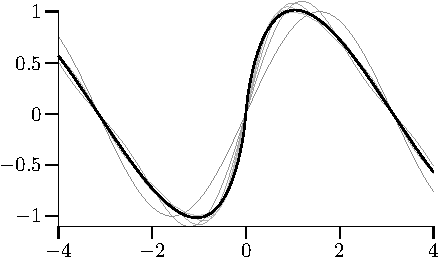
\includegraphics{figures/fouriersern2}
\caption{Plot of 
$\sum_{n=1}^\infty \frac{\sin(n x)}{n^2}$ including
the first 8 partial sums in various shades of gray.\label{fig:fouriersern2}}
\end{myfigureht}

\begin{example}
The series
\begin{equation*}
\sum_{n=0}^\infty \frac{1}{n!} x^n
\end{equation*}
converges uniformly on any bounded interval.
Take the interval $[-r,r] \subset \R$ (any bounded interval
is contained in such an interval)
\begin{equation*}
\abs{\frac{1}{n!} x^n} \leq 
\frac{r^n}{n!}
\end{equation*}
and we have seen before that
$\sum_{n=1}^\infty \frac{r^n}{n!}$ converges, for example by the ratio test.
\end{example}

Now we would love to say something about the limit.  For example, is it
continuous?


\begin{prop} \label{prop:uniformswitch}
Let $(X,d_X)$ and $(Y,d_Y)$ be metric spaces, and let
$f_n \colon X \to Y$ be functions.
Suppose $Y$ is complete metric space.
Suppose $\{ f_n \}$ converges uniformly to $f \colon X \to \C$.  
Let $\{ x_k \}$ be a sequence in $X$ and $x = \lim \, x_k$.  Suppose
that
\begin{equation*}
a_n = \lim_{k \to \infty} f_n(x_k)
\end{equation*}
exists for all $n$.  Then
$\{a_n\}$ converges and 
\begin{equation*}
\lim_{k \to \infty} f(x_k) = \lim_{n\to\infty} a_n
\end{equation*}
\end{prop}

In other words
\begin{equation*}
\lim_{k \to \infty} \lim_{n\to\infty} f_n(x_k) =
\lim_{n \to \infty} \lim_{k\to\infty} f_n(x_k) .
\end{equation*}

\begin{proof}
First we have to show that $\{ a_n \}$ converges.  As
$\{ f_n \}$ converges uniformly it is uniformly Cauchy. 
Let $\epsilon > 0$ be given.  There is
an $M$ such that for all $m,n \geq M$ we have
\begin{equation*}
d_Y\bigl(f_n(x_k),f_m(x_k)\bigr) < \epsilon \qquad \text{for all $k$} .
\end{equation*}
As a metric is automatically continuous we can let $k$ go to infinity
to find
\begin{equation*}
d_Y(a_n,a_m) \leq \epsilon .
\end{equation*}
Hence $\{a_n\}$ is Cauchy and converges since $Y$ is complete.  Write
$a := \lim_{n\to\infty} a_n$.

Find a $k \in \N$ such that
\begin{equation*}
d_Y\bigl(f_k(p),f(p)\bigr) < \nicefrac{\epsilon}{3}
\end{equation*}
for all $p \in X$.  Assume $k$ is large enough
so that
\begin{equation*}
d_Y(a_k,a) < \nicefrac{\epsilon}{3}  .
\end{equation*}
Find an $N \in \N$ such that for $m \geq N$,
\begin{equation*}
d_Y\bigl(f_k(x_m),a_k\bigr) < \nicefrac{\epsilon}{3}  .
\end{equation*}
Then for
$m \geq N$,
\begin{equation*}
d_Y\bigl(f(x_m),a\bigr)
\leq
d_Y\bigl(f(x_m),f_k(x_m)\bigr)
+
d_Y\bigl(f_k(x_m),a_k\bigr)
+
d_Y\bigl(a_k,a\bigr)
<
\nicefrac{\epsilon}{3} +
\nicefrac{\epsilon}{3} +
\nicefrac{\epsilon}{3} = \epsilon . \qedhere
\end{equation*}
\end{proof}

Immediately we obtain a corollary about continuity.

\begin{cor} \label{cor:metricuniformcontinuous}
Let $X$ and $Y$ be metric spaces such that $Y$ is Cauchy complete.
Let $f_n \colon X \to Y$ be continuous functions
such that
$\{ f_n \}$ converges uniformly to $f \colon X \to Y$.  
Then $f$ is continuous.
\end{cor}

Converse is not true.  Just because the limit is continuous doesn't mean
that the convergence is uniform.  For example:
$f_n \colon (0,1) \to \R$ defined by $f_n(x) := x^n$ converge to
the zero function, but not uniformly.  However, if we add extra conditions
on the sequence can obtain a partial converse such as Dini's theorem,
\volIref{see Exercise 6.2.10 from volume I}.

Assuming the exercise that for a compact $X$, $C(X,\C)$ is a metric space with
the uniform norm (actually a normed vector space).  We have just shown that
it is Cauchy complete.  \propref{prop:unifcauchymetric} says that a Cauchy
sequence in $C(X,\C)$ converges to some function,
and \corref{cor:metricuniformcontinuous} shows that the limit is in fact
continuous and hence in $C(X,\C)$.

\begin{cor}
Let $(X,d)$ be a compact metric space, then $C(X,\C)$ is a Cauchy
complete metric space.
\end{cor}

\begin{example}
We have seen that the example Fourier series 
\begin{equation*}
\sum_{n=1}^\infty \frac{\sin(nx)}{n^2}
\end{equation*}
converges uniformly and hence is continuous (as is visible
in \figureref{fig:fouriersern2}).
\end{example}

\subsection{Integration}

\begin{prop} \label{prop:complexlimitswapintegral}
Suppose $f_n \colon [a,b] \to \C$
are Riemann integrable and suppose that $\{ f_n \}$ converges
uniformly to $f \colon [a,b] \to \C$.  Then $f$ is Riemann integrable
and
\begin{equation*}
\int_a^b f = \lim_{n\to \infty} \int_a^b f_n
\end{equation*}
\end{prop}

Since the integral of a complex-valued function is just the integral of
the real and imaginary parts separately,
the proof follows directly by the results of \volIref{chapter 6 of volume I}.  We
leave the details as an exercise.

\begin{cor}
Suppose $f_n \colon [a,b] \to \C$
are Riemann integrable and suppose that
\begin{equation*}
\sum_{n=1}^\infty f_n(x)
\end{equation*}
converges uniformly.  Then the series is Riemann integrable on $[a,b]$
and
\begin{equation*}
\int_a^b \sum_{n=1}^\infty f_n(x) ~dx
=
\sum_{n=1}^\infty \int_a^b f_n(x) ~dx
\end{equation*}
\end{cor}

\begin{example}
Let us show how to integrate a Fourier series.
\begin{equation*}
\int_{0}^x \sum_{n=1}^\infty \frac{\cos(nt)}{n^2} ~dt
=
\sum_{n=1}^\infty \int_{0}^x \frac{\cos(nt)}{n^2}~dt
=
\sum_{n=1}^\infty \frac{\sin(nx)}{n^3}
\end{equation*}
The swapping of integral and sum is possible because of uniform convergence,
which we have proved before using the $M$ test.
\end{example}

Note that we can swap integrals and limits under far less stringent hypotheses,
but for that we would need a stronger integral than the Riemann integral.
E.g.\ the Lebesgue integral.

\subsection{Differentiation}

For complex-valued functions, define the
\emph{derivative}\index{derivative!complex-valued function}
of $f \colon [a,b] \to
\C$ where $f(x) = u(x)+iv(x)$ as
\begin{equation*}
f'(x) := u'(x)+iv'(x) .
\end{equation*}
This definition is consistent with the definition for vector valued
functions as the complex number that is the derivative of $f$ gives rise to
a real-linear operator on $\R^2$.

The proof of the following theorem is to apply the corresponding theorem for
real functions to $u$ and $v$, and is left as an exercise.

\begin{thm} \label{thm:dersconvergecomplex}
Let $I \subset \R$ be a bounded interval and let
$f_n \colon I \to \C$ be continuously differentiable functions.
Suppose $\{ f_n' \}$ converges uniformly to $g \colon I \to \C$,
and suppose $\{ f_n(c) \}_{n=1}^\infty$ is a
convergent sequence for some $c \in I$.  Then $\{ f_n \}$ converges uniformly to 
a continuously differentiable function $f \colon I \to \C$, and $f' = g$.
\end{thm}

%FIXME: an example perhaps definitely using complex

\begin{example}
Let us construct a continuous nowhere differentiable function.
Such functions are often called Weierstrass functions, although this
particular one is a different example than what Weierstrass gave.

Define
\begin{equation*}
\varphi(x) :=\sabs{x} \qquad \text{for $x \in [-1,1]$} .
\end{equation*}
We extend the definition to all of $\R$ by making $\varphi$ 2-periodic,
that is, we decree that
$\varphi(x) = \varphi(x+2)$.  The function $\varphi \colon \R \to \R$
is continuous,in fact $\sabs{\varphi(x)-\varphi(y)} \leq \sabs{x-y}$ (why?).
See \figureref{fig:triangwave}.
\begin{myfigureht}
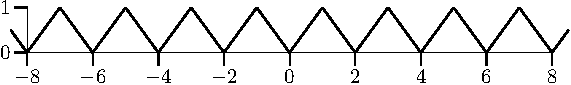
\includegraphics{figures/triangwave}
\caption{The 2-periodic function $\varphi$.\label{fig:triangwave}}
\end{myfigureht}

As $\sum {\left(\frac{3}{4}\right)}^n$ converges and $\sabs{\varphi(x)} \leq
1$ for all $x$, we have by the M-test that
\begin{equation*}
f(x) := \sum_{n=0}^\infty 
{\left(\frac{3}{4}\right)}^n \varphi(4^n x)
\end{equation*}
converges uniformly and hence is continuous.  We claim that this $f \colon
\R \to \R$ is nowhere differentiable.
See \figureref{fig:nowherediff}.

\begin{myfigureht}
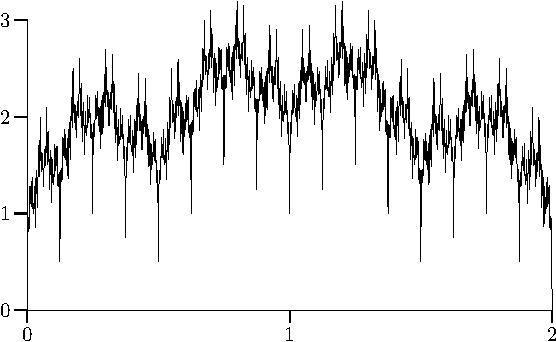
\includegraphics{figures/nowherediff}
\caption{Plot of the nowhere differentiable function $f$.\label{fig:nowherediff}}
\end{myfigureht}

Fix $x$ and
define
\begin{equation*}
\delta_m := \pm \frac{1}{2} 4^{-m}
\end{equation*}
where the sign is chosen in such a way so that there is no integer
between $4^m x$ and $4^m(x+\delta_m)$, which can be done
since $4^m\sabs{\delta_m} = \frac{1}{2}$.  Fix $m$ for a moment.

Let
\begin{equation*}
\gamma_{n} :=
\frac{\varphi\bigl(4^n(x+\delta_m)\bigr)-\varphi(4^nx)}{\delta_m} .
\end{equation*}
If $n > m$, then $4^n\delta_m$ is an even integer.  As $\varphi$
is 2-periodic we get that $\gamma_n = 0$.

There is no integer between 
$4^mx\pm\nicefrac{1}{2}$ and $4^mx$, so
$\abs{\varphi(4^mx\pm\nicefrac{1}{2})-\varphi(4^mx)} =
\abs{4^mx\pm\nicefrac{1}{2}-4^mx} = \nicefrac{1}{2}$.  Therefore
\begin{equation*}
\sabs{\gamma_m} =
\abs{
\frac{\varphi(4^mx\pm\nicefrac{1}{2})-\varphi(4^mx)}{\pm (\nicefrac{1}{2}) 4^{-m}}
}
= 4^m .
\end{equation*}
Similarly, if $n < m$ we, since $\sabs{\varphi(s) -\varphi(t)} \leq
\sabs{s-t}$,
\begin{equation*}
\sabs{\gamma_n} =
\abs{\frac{\varphi\bigl(4^nx\pm(\nicefrac{1}{2})4^{n-m}\bigr)-\varphi(4^nx)}{\pm
(\nicefrac{1}{2}) 4^{-m}}}
\leq
\abs{\frac{\pm(\nicefrac{1}{2})4^{n-m}}{\pm (\nicefrac{1}{2}) 4^{-m}}} = 4^n
.
\end{equation*}

And so
\begin{equation*}
\begin{split}
\abs{
\frac{f(x+\delta_m)-f(x)}{\delta_m}
}
& =
\abs{
\sum_{n=0}^\infty 
{\left(\frac{3}{4}\right)}^n
\frac{\varphi\bigl(4^n(x+\delta_m)\bigr)-\varphi(4^nx)}{\delta_m}
}
=
\abs{
\sum_{n=0}^\infty 
{\left(\frac{3}{4}\right)}^n
\gamma_n
}
\\
& =
\abs{
\sum_{n=0}^m 
{\left(\frac{3}{4}\right)}^n
\gamma_n
}
\\
& \geq
\abs{
{\left(\frac{3}{4}\right)}^m
\gamma_m}
-
\abs{
\sum_{n=0}^{m-1} 
{\left(\frac{3}{4}\right)}^n
\gamma_n
}
\\
& \geq
3^m
-
\sum_{n=0}^{m-1} 
3^n
=
3^m
-
\frac{3^{m}-1}{3-1}
=
\frac{3^m +1}{2} .
\end{split}
\end{equation*}
It is obvious that $\delta_m \to 0$ as $m \to \infty$, but $\frac{3^m+1}{2}$
goes to infinity.  Hence $f$ cannot be differentiable at $x$.

We will see later that such an $f$ is a uniform limit of not just
differentiable functions but actually it is the uniform limit of
polynomials.
\end{example}

\subsection{Exercises}

\begin{exercise}
Prove \propref{prop:uniformconvbounded}.
\end{exercise}

\begin{exercise}
Prove \propref{prop:unifcauchymetric}.
\end{exercise}

\begin{exercise}
Suppose $(X,d)$ is a compact metric space.
Prove that $\snorm{\cdot}_u$ is a norm on the vector space of
continuous complex-valued functions $C(X,\C)$.
\end{exercise}

\begin{exercise}
Prove \thmref{thm:dersconvergecomplex}.
\end{exercise}

\begin{exercise}
Prove \propref{prop:complexlimitswapintegral} by reducing to the real
result.
\end{exercise}

%%%%%%%%%%%%%%%%%%%%%%%%%%%%%%%%%%%%%%%%%%%%%%%%%%%%%%%%%%%%%%%%%%%%%%%%%%%%%%

\sectionnewpage
\section{Equicontinuity and the Arzel{\` a}--Ascoli theorem}
\label{sec:arzelaascoli}

\sectionnotes{2 lectures}

We would like an analogue of Bolzano-Weierstrass.  Something to the tune of
``every bounded
sequence of functions (with some property) has a convergent subsequence''.
Matters are not
as simple even for continuous functions. 
Not every bounded sequence in the metric space $C([0,1],\R)$ has
a convergent subsequence (see below).

\begin{defn}
Let $X$ be any set.
Let $f_n \colon X \to \C$ be functions in a sequence.  We say that
$\{ f_n \}$
is \emph{\myindex{pointwise bounded}} if for every $x \in X$, there is an $M_x \in \R$
such that
\begin{equation*}
\sabs{f_n(x)} \leq M_x \qquad \text{for all $n \in \N$} .
\end{equation*}
We say that
$\{ f_n \}$
is \emph{\myindex{uniformly bounded}} if there is an $M \in \R$
such that
\begin{equation*}
\sabs{f_n(x)} \leq M \qquad \text{for all $n \in \N$ and all $x \in X$}.
\end{equation*}
\end{defn}

Note that uniform boundedness is the same as boundedness in the metric space
$C(X,\C)$ (here $X$ is a compact metric space).

\begin{example}
There exist sequences of 
continuous functions
on $[0,1]$ that are uniformly bounded but contain no subsequence converging
even pointwise.  Let us state without proof that $f_n(x) := \sin (2\pi n x)$ is one
such sequence.
\end{example}

\begin{example}
We also have that $f_n(x) := x^n$ is a sequence of functions on $[0,1]$
that is uniformly bounded, but contains no sequence that converges
uniformly,
although the sequence converges pointwise.
\end{example}

When the domain is countable, matters are easier.   The proof uses
a very common and useful diagonal argument.

\begin{thm} \label{thm:subsequenceoncountableX}
Let $X$ be a countable set and $f_n \colon X \to \C$ give a pointwise bounded
sequence of functions, then $\{ f_n \}$ has a subsequence that converges
pointwise.
\end{thm}

\begin{proof}
Let $\{ x_k \}$ be an enumeration of the elements of $X$.
The sequence $\{ f_n(x_1) \}_{n=1}^\infty$ is bounded and hence
we have a subsequence which we denote by
$f_{1,k}$ such that $\{ f_{1,k}(x_1) \}$ converges.
Next $\{ f_{1,k}(x_2) \}$ has a subsequence that converges and
we denote that subsequence by
$\{ f_{2,k}(x_2) \}$.  In general we have a sequence $\{ f_{m,k}
\}_{k=1}^\infty$
that makes $\{ f_{m,k}(x_j) \}_{k=1}^\infty$ converge for all $j \leq m$ and we 
let $\{ f_{m+1,k} \}_{k=1}^\infty$ be the subsequence of $\{ f_{m,k}
\}_{k=1}^\infty$
such that
$\{ f_{m+1,k}(x_{m+1}) \}_{k=1}^\infty$ converges (and hence it converges for all
$x_j$ for $j=1,\ldots,m+1$) and we can rinse and repeat.

If $X$ is finite we are done.  If $X$ is countably infinite,
we pick the sequence
$\{ f_{k,k} \}$.  This is a subsequence of the original sequence $\{ f_n \}$
of course.  Also for any $m$,
except for the first $m$ terms $\{ f_{k,k} \}$ is a subsequence of $\{ f_{m,k}
\}_{k=1}^\infty$
and hence for any $m$ the sequence $\{ f_{k,k}(x_m) \}_{k=1}^\infty$ converges.
\end{proof}

For larger than countable sets,
we need the functions of the sequence to be related.  We look at
continuous functions, and the concept we need is equicontinuity.

\begin{defn}
Let $X$ be a metric space.
A family $\sF$ of functions $f \colon X \to \C$ is said to be
\emph{\myindex{equicontinuous}} on $X$ if for every $\epsilon > 0$, there is a $\delta > 0$
such that if $x, y \in X$ with $d(x,y) < \delta$ we have
\begin{equation*}
\sabs{f(x)-f(y)} < \epsilon \qquad \text{ for all $f \in \sF$} .
\end{equation*}
\end{defn}

One obvious fact is that if $\sF$ is equicontinuous, then every element of
$f$ is uniformly continuous.  Also obvious is that any finite set of
uniformly continuous functions is an equicontinuous family.  Of course the
interesting case is when $\sF$ is an infinite family such as a sequence of
functions.  Equicontinuity of a sequence
is closely related to uniform convergence.

\begin{prop}
Suppose $(X,d)$ is a compact metric space,
$f_n \in C(X,\C)$, and $\{ f_n \}$
converges uniformly, then $\{ f_n \}$ is equicontinuous.
\end{prop}

\begin{proof}
Let $\epsilon > 0$ be given.
As $f_n$ converge uniformly, there is an integer $N$ such that for
all $n \geq N$ we have
\begin{equation*}
\sabs{f_n(x)-f_N(x)} < \nicefrac{\epsilon}{3} \qquad \text{for all $x \in X$}.
\end{equation*}
As $X$ is compact and so continuous means
uniformly continuous,
$\{ f_1,f_2,\ldots,f_N \}$ is a finite set of uniformly continuous
functions.  And so, as we mentioned above, it is an equicontinuous family.  Hence
there is a $\delta > 0$ such that
\begin{equation*}
\sabs{f_j(x)-f_j(y)} < \nicefrac{\epsilon}{3} < \epsilon
\end{equation*}
whenever $d(x,y) < \delta$ and $1 \leq j \leq N$.

Now take $n > N$.  Then for $d(x,y) < \delta$ we have
\begin{equation*}
\sabs{f_n(x)-f_n(y)}
\leq
\sabs{f_n(x)-f_N(x)}
+
\sabs{f_N(x)-f_N(y)}
+
\sabs{f_N(y)-f_n(y)}
<
\nicefrac{\epsilon}{3}
+
\nicefrac{\epsilon}{3}
+
\nicefrac{\epsilon}{3}
=\epsilon . \qedhere
\end{equation*}
\end{proof}

\begin{prop}
A compact metric space $X$ contains a countable dense subset.
\end{prop}

\begin{proof}
For each $n \in \N$ we have that there are finitely many
balls of radius $\nicefrac{1}{n}$ that cover $X$ (as $X$ is compact). That is,
for every $n$, there exists
a finite set of points $x_{n,1},x_{n,2},\ldots,x_{n,k_n}$ such that
\begin{equation*}
X= \bigcup_{j=1}^{k_n} B(x_{n,j},\nicefrac{1}{n})
\end{equation*}
So consider the set $S$ of all the points $x_{n,j}$.  As $S$ is a countable
union of finite sets and therefore countable.  For every $x \in X$
and every $\epsilon > 0$, there exists an $n$ such that
$\nicefrac{1}{n} < \epsilon$ and an $x_{n,j} \in S$ such that
\begin{equation*}
x \in B(x_{n,j},\nicefrac{1}{n}) \subset B(x_{n,j},\epsilon) .
\end{equation*}
Hence $x \in \overline{S}$, so $\overline{S} = X$ and $S$ is dense.
\end{proof}

We are now ready for the main result of this section,
the Arzel\`a--Ascoli theorem about existence of convergent subsequences.

\begin{thm}[Arzel\`a--Ascoli]\index{Arzel\`a--Ascoli theorem}
Let $(X,d)$ be a compact metric space, $f_n \in C(X,\C)$, and let $\{ f_n \}$
be pointwise bounded and equicontinuous.  Then
$\{f_n\}$ is uniformly bounded and $\{ f_n \}$ contains a uniformly
convergent subsequence.
\end{thm}

Basically, an equicontinuous sequence in the metric space
$C(X,\C)$ that is pointwise bounded
is bounded (in $C(X,\C)$) and furthermore contains a convergent
subsequence in $C(X,\C)$.

\begin{proof}
Let us first show that the sequence is uniformly bounded.

By equicontinuity we have that there is a $\delta > 0$
such that for all $x \in X$
\begin{equation*}
B(x,\delta) \subset f_n^{-1}\bigl(B(f_n(x),1)\bigr) .
\end{equation*}
Now $X$ is compact, so there exists $x_1,x_2,\ldots,x_k$
such that
\begin{equation*}
X = \bigcup_{j=1}^k B(x_j,\delta)
\end{equation*}
As $\{ f_n \}$ is pointwise bounded there exist $M_1,M_2,\ldots,M_k$
such that for $j=1,\ldots,k$ we have
\begin{equation*}
\sabs{f_n(x_j)} \leq M_j
\end{equation*}
for all $n$.  Let $M = 1+ \max \{ M_1,\ldots,M_k \}$.  Now given any
$x \in X$, there is a $j$ such that $x \in B(x_j,\delta)$.  Therefore,
for all $n$ we have
$x \in f_n^{-1}\bigl(B(f_n(x_j),1)\bigr)$ or in other words
\begin{equation*}
\sabs{f_n(x)-f_n(x_j)} < 1 .
\end{equation*}
By reverse triangle inequality,
\begin{equation*}
\sabs{f_n(x)} < 1+ \sabs{f_n(x_j)} \leq 1+M_j \leq M .
\end{equation*}
And as $x$ was arbitrary, $\{f_n\}$ is uniformly bounded.


Next, pick a countable dense set $S$.  By \thmref{thm:subsequenceoncountableX}, we find
a subsequence $\{ f_{n_j} \}$ that converges pointwise on $S$.
Write $g_j = f_{n_j}$ for simplicity.  Note that $\{ g_n \}$ is 
equicontinuous.

Let $\epsilon > 0$ be given, then pick $\delta > 0$
such that for all $x \in X$
\begin{equation*}
B(x,\delta) \subset g_n^{-1}\bigl(B(g_n(x),\nicefrac{\epsilon}{3})\bigr).
\end{equation*}
By density of $S$, every $x \in X$ is in some $B(y,\delta)$
for some $y \in S$, and by compactness of $X$,
there is a finite subset $\{ x_1,\ldots,x_k \}$ of $S$
such that
\begin{equation*}
X = \bigcup_{j=1}^k B(x_j,\delta) .
\end{equation*}
Now as there are finitely many points and we know that $\{ g_n \}$
converges pointwise on $S$, there exists a single $N$ such that for 
all $n,m \geq N$ we have for all $j=1,\ldots,k$
\begin{equation*}
\sabs{g_n(x_j)-g_m(x_j)} < \nicefrac{\epsilon}{3} .
\end{equation*}

Let $x \in X$ be arbitrary.  There is some $j$ such that
$x \in B(x_j,\delta)$ and so we have for all $i \in \N$
\begin{equation*}
\sabs{g_i(x)-g_i(x_j)} < \nicefrac{\epsilon}{3},
\end{equation*}
and so $n,m \geq N$ that
\begin{equation*}
\sabs{g_n(x)-g_m(x)} \leq
\sabs{g_n(x)-g_n(x_j)} +
\sabs{g_n(x_j)-g_m(x_j)} +
\sabs{g_m(x_j)-g_m(x)} <
\nicefrac{\epsilon}{3} +
\nicefrac{\epsilon}{3} +
\nicefrac{\epsilon}{3} = \epsilon . \qedhere
\end{equation*}
\end{proof}

\begin{cor}
Let $X$ be a compact metric space.
Let $S \subset C(X,\C)$ be a closed, bounded and equicontinuous set.
Then $S$ is compact.
\end{cor}

The theorem says that $S$
is sequentially compact and we know that means
compact in a metric space.
Recall that the closed unit ball in $C([0,1],\R)$ (and therefore also in
$C([0,1],\C)$) is not compact.
Hence it cannot be an equicontinuous set.

\begin{cor}
Suppose $\{ f_n \}$ is a sequence of differentiable functions on $[a,b]$,
$\{ f_n' \}$ is uniformly bounded, and there is an
$x_0 \in [a,b]$ such that $\{ f_n(x_0) \}$ is bounded.
Then there exists a uniformly convergent
subsequence $\{ f_{n_j} \}$.
\end{cor}

\begin{proof}
The trick is to use the mean value theorem.  If $M$ is the uniform bound on
$\{ f_n' \}$, then we have by the mean value theorem
\begin{equation*}
\sabs{f_n(x)-f_n(y)} \leq M \sabs{x-y} .
\end{equation*}
So all the $f_n$ are Lipschitz with the same constant and hence
equicontinuous.

Suppose $\sabs{f_n(x_0)} \leq M_0$ for all $n$.
By the inverse triangle inequality, for all $x \in [a,b]$
\begin{equation*}
\sabs{f_n(x)} \leq \sabs{f_n(x_0)}+ \sabs{f_n(x)-f_n(x_0)} \leq M_0+ M \sabs{x-x_0}
\leq M_0 + M(b-a) .
\end{equation*}
So $\{ f_n \}$ is uniformly bounded.
We apply Arzel\`a--Ascoli to find the subsequence.
\end{proof}

A consequence of the above corollary and the fundamental theorem of calculus
is that given some fixed $g \in
C([0,1],\C)$,
the set of functions
\begin{equation*}
\left\{
F \in C([0,1],\C) : F(x) = \int_0^x g(t) f(t)~dt,~ f \in C([0,1],\C),~
\snorm{f}_u \leq 1
\right\}
\end{equation*}
has compact closure, usually called
\emph{\myindex{relatively compact}} (exercise).
That is, the operator $T \colon C([0,1],\C) \to C([0,1],\C)$ given by
\begin{equation*}
T\bigl(f\bigr) (x) := F(x) = \int_0^x g(t) f(t)~dt
\end{equation*}
takes the unit ball centered at 0 in $C([0,1],\C)$ into a relatively compact set.  We often
say that this means that the operator is compact, and such operators are very
important (and very useful).

\subsection{Exercises}

\begin{exercise}
Let $(X,d)$ be a compact metric space, $C > 0$, $0 < \alpha \leq 1$, and
suppose $f_n \colon X \to \C$ are functions such as
$\abs{f_n(x)-f_n(y)} \leq C {d(x,y)}^\alpha$ for all $x,y \in X$ and
$n \in \N$.  Suppose also that there is a point $p \in X$ such that
$f_n(p) = 0$.
Show that there exists a uniformly convergent subsequence converging to
an $f \colon X \to \C$ that also satisfies $f(p) = 0$ and
$\abs{f(x)-f(y)} \leq C {d(x,y)}^\alpha$.
\end{exercise}

\begin{exercise}
Show that the operator $T \colon C([0,1],\C) \to C([0,1],\C)$ given by
\begin{equation*}
T\bigl(f\bigr) (x) := F(x) = \int_0^x g(t) f(t)~dt
\end{equation*}
takes the unit ball centered at 0 in $C([0,1],\C)$ into a
relatively compact set.
\end{exercise}

\begin{exercise}
Suppose $S^1 \subset \C$ is the unit circle, that is the set where
$\sabs{z}=1$.  Suppose the continuous functions
$f_n \colon S^1 \to \C$ are uniformly bounded.
Let $\gamma \colon [0,1] \to \S^1$ be a parametrization of $S^1$,
and $g(z,w)$ a continuous function on $C(0,1) \times S^1$.  Define
the functions $F_n \colon C(0,1) \to \C$ by
the path integral (See \sectionref{sec:pathintegral})
\begin{equation*}
F_n(z) : = \int_\gamma f_n(w)\, g(z,w) ~ ds(w) . 
\end{equation*}
Show that $\{ F_n \}$ has a uniformly convergent subsequence.
\end{exercise}


%%%%%%%%%%%%%%%%%%%%%%%%%%%%%%%%%%%%%%%%%%%%%%%%%%%%%%%%%%%%%%%%%%%%%%%%%%%%%%

\sectionnewpage
\section{The Stone--Weierstrass theorem}
\label{sec:stoneweier}

\sectionnotes{2 lectures}

\subsection{Weierstrass approximation}

Perhaps surprisingly, even a very badly behaving continuous function is really
just a uniform limit of polynomials.  We cannot really get any ``nicer'' as
a function than a polynomial.

\begin{thm}[Weierstrass approximation theorem]
If $f \colon [a,b] \to \C$ is continuous, then there exists a sequence $\{
p_n \}$ of polynomials converging to $f$ uniformly on $[a,b]$.
Furthermore, if $f$ is real-valued, we can find real-valued $p_n$.
\end{thm}

\begin{proof}
For $x \in [0,1]$ define
\begin{equation*}
g(x) := f\bigl((b-a)x+a\bigr)-f(a) - x\bigl(f(b)-f(a)\bigr) .
\end{equation*}
If we can prove the theorem for $g$ and find the $\{ p_n \}$ for $g$,
we can prove it for $f$ since we simply
composed with an invertible affine function and added an affine
function to $f$, so we can easily reverse the process and apply that to our
$p_n$, to obtain polynomials approximating $f$.

So $g$ is defined on $[0,1]$ and $g(0)=g(1)=0$.  We now assume that
$g$ is defined on the whole real line for simplicity by defining
$g(x) := 0$ if $x < 0$ or $x > 1$.

Define
\begin{equation*}
c_n := {\left( \int_{-1}^1 {(1-x^2)}^n~dx \right)}^{-1} ,
\qquad
q_n(x) := c_n (1-x^2)^n
\end{equation*}
so that $\int_{-1}^1 q_n(x)~dx = 1$.
See \figureref{fig:weierqn}.

\begin{myfigureht}
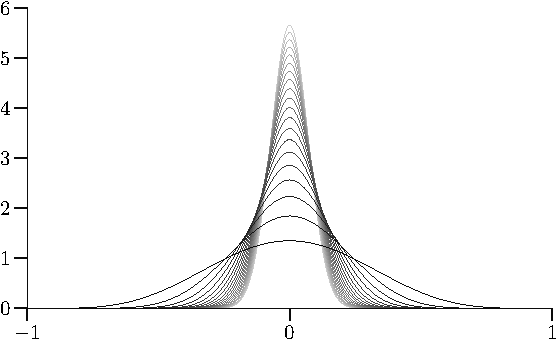
\includegraphics{figures/weierqn}
\caption{Plot of the approximate delta functions $q_n$ on $[-1,1]$ for
$n=5,10,15,20,\ldots,100$ with higher $n$ in lighter shade.\label{fig:weierqn}}
\end{myfigureht}

The functions $q_n$ are peaks around 0 (ignoring what happens outside
of $[-1,1]$) that get narrower and narrower, but the area underneath is
always 1.
A classic approximation idea
is to do a \emph{\myindex{convolution}} integral with peaks like this.
That is we 
write for $x \in [0,1]$,
\begin{equation*}
p_n(x) = \int_{0}^1 g(t)q_n(x-t) ~dt \quad \left( = \int_{-\infty}^\infty
g(t)q_n(x-t) ~dt \right) .
\end{equation*}
The idea of this convolution is that we do a ``weighted average'' of the
function $g$ around the point $x$ using $q_n$ as the weight.
See \figureref{fig:approxdeltaconv}.

\begin{myfigureht}
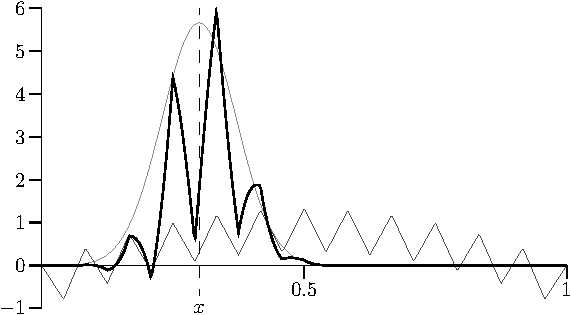
\includegraphics{figures/approxdeltaconv}
\caption{For $x=0.3$, the plot of $q_{100}(x-t)$ (light gray peak centered
at $x$), some continuous function
$g(t)$ (the jagged line) and the product $g(t)q_{100}(x-t)$ (the bold line).\label{fig:approxdeltaconv}}
\end{myfigureht}

As $q_n$ is a narrow peak, the integral
only sees the values of $g$ that are
close to $x$ and it does the weighted average of them.
When the peak gets narrower, we compute this average closer to $x$
and we expect the result to get closer to the value of $g(x)$.  Really we are
approximating what is called a delta function\footnote{which is not actually
a function} (don't worry if you have not
heard of this concept),
and functions like $q_n$ are often called
\emph{approximate delta functions}\index{approximate delta function}.
We could really do this with any polynomial that looks like a little peak
near zero.  This just happens to be the simplest one.
We only need this behavior on $[-1,1]$ as the convolution sees nothing
further than this as $g$ is zero outside $[0,1]$.

Because $q_n$ is a polynomial we can write
\begin{equation*}
q_n(x-t) = a_0(t) + a_1(t)x + \cdots + a_{2n}(t) x^{2n}
\end{equation*}
for some functions $a_k(t)$.
Since the integral is in terms of $t$, the $x$s just pop out
by linearity of the integral,
and so we obtain that $p_n$ is a polynomial in $x$.
Finally if $g(t)$ is real-valued then the functions $g(t)a_j(t)$ are
real-valued and hence $p_n$ has real coefficients
(proving the ``furthermore'' part of the theorem).

We still need to prove that the limit of the $p_n$ is $g$.  First we need
to get some handle on the
size of $c_n$.  For $x \in [0,1]$,
\begin{equation*}
{(1-x^2)}^n \geq (1-nx^2) .
\end{equation*}
This fact is an application of Bernoulli's inequality or can be 
prove directly:
the two expressions are equal at $x=0$ and 
$\frac{d}{dx}\left({(1-x^2)}^n - (1-nx^2)\right)
=-2nx{(1-x^2)}^{n-1}+2nx$, which is nonnegative for $x \in [0,1]$.
Furthermore $1-nx^2 \geq 0$ for $x \in [0,\nicefrac{1}{\sqrt{n}}]$.
\begin{multline*}
c_n^{-1}  = \int_{-1}^1 {(1-x^2)}^n ~ dx
= 2\int_0^1 {(1-x^2)}^n ~ dx \\
\geq 2\int_0^{1/\sqrt{n}} {(1-x^2)}^n ~ dx
\geq 2\int_0^{1/\sqrt{n}} (1-nx^2)  ~ dx
= \frac{4}{3\sqrt{n}}
> \frac{1}{\sqrt{n}} .
\end{multline*}
so $c_n < \sqrt{n}$.

Let's see how small $g$ is if we ignore some small bit around the origin,
which is where the peak is.
Given any $\delta > 0$, $\delta < 1$, we have for $\delta \leq \sabs{x} \leq
1$
\begin{equation*}
q_n(x) \leq \sqrt{n}{(1-\delta^2)}^n .
\end{equation*}
Then it is easy to see (e.g.\ by the ratio test) that
$\sqrt{n}{(1-\delta^2)}^n$ goes to 0 as $n$ goes to infinity.
The function $q_n$ is even, $q_n(t) = q_n(-t)$, and $g$
is zero outside of $[0,1]$.
So for $x \in [0,1]$,
\begin{equation*}
p_n(x) = 
\int_{0}^1 g(t)q_n(x-t)  ~ dt
=
\int_{-x}^{1-x} g(t+x)q_n(-t)  ~ dt
=
\int_{-1}^{1} g(t+x)q_n(t)  ~ dt .
\end{equation*}

Let $\epsilon > 0$ be given.
As $[-1,2]$ is compact and $g$ is continuous on $[-1,2]$, we have that $g$ is uniformly continuous.
Pick $0 < \delta < 1$ such that if
$\sabs{x-y} < \delta$ (and $x,y \in [-1,2]$) then
\begin{equation*}
\sabs{g(x)-g(y)} < \frac{\epsilon}{2} .
\end{equation*}

Let $M$ be such that $\sabs{g(x)} \leq M$ for all $x$.  Let $N$ be
such that for all $n \geq N$,
\begin{equation*}
4M\sqrt{n}{(1-\delta^2)}^n < \frac{\epsilon}{2} .
\end{equation*}

Note that 
$\int_{-1}^1 q_n(t) ~ dt = 1$ and $q_n(x) \geq 0$ on $[-1,1]$ so
\begin{equation*}
\begin{split}
\sabs{p_n(x)-g(x)} & =
\abs{\int_{-1}^1 g(t+x)q_n(t) ~ dt
-g(x)\int_{-1}^1 q_n(t) ~ dt} \\
& =
\abs{\int_{-1}^1 \bigl(g(t+x)-g(x)\bigr)q_n(t) ~ dt} \\
& \leq
\int_{-1}^1 \sabs{g(t+x)-g(x)} q_n(t) ~ dt \\
& =
\int_{-1}^{-\delta} \sabs{g(t+x)-g(x)} q_n(t) ~ dt
+
\int_{-\delta}^{\delta} \sabs{g(t+x)-g(x)} q_n(t) ~ dt
\\
& \phantom{\leq} +
\int_{\delta}^1 \sabs{g(t+x)-g(x)} q_n(t) ~ dt \\
& \leq
2M
\int_{-1}^{-\delta} q_n(t) ~ dt
+
\frac{\epsilon}{2}
\int_{-\delta}^{\delta} q_n(t) ~ dt
+
2M
\int_{\delta}^1 q_n(t) ~ dt \\
& \leq
2M\sqrt{n}{(1-\delta^2)}^n(1-\delta)
+
\frac{\epsilon}{2}
+
2M\sqrt{n}{(1-\delta^2)}^n(1-\delta) \\
& <
4M\sqrt{n}{(1-\delta^2)}^n
+
\frac{\epsilon}{2}
< \epsilon . \qedhere
\end{split}
\end{equation*}
\end{proof}

%Think about the consequences of the theorem.  If you have any property that
%gets preserved under uniform convergence and it is true for polynomials,
%then it must be true for all continuous functions.

Let us note an immediate application of the Weierstrass theorem.  We have
already seen that countable dense subsets can be very useful.

\begin{cor}
The metric space $C([a,b],\C)$ contains a countable dense subset.
\end{cor}

\begin{proof}
Without loss of generality suppose that we are dealing with $C([a,b],\R)$
(why?).
The real polynomials are dense in $C([a,b],\R)$.  If we show that
any real polynomial can be approximated by polynomials with rational
coefficients, we are done.  This is because there are only countably many
rational numbers and so there are only countably many polynomials with
rational coefficients (a countable union of countable sets is still
countable).

Further without loss of generality, suppose $[a,b]=[0,1]$.  Let
\begin{equation*}
p(x) = \sum_{k=0}^n a_k x^k
\end{equation*}
be a polynomial of degree $n$ where $a_k \in \R$.  Given $\epsilon > 0$, pick $b_k \in \Q$
such that $\sabs{a_k-b_k} < \frac{\epsilon}{n+1}$.  Then
if we let
\begin{equation*}
q(x) = \sum_{k=0}^n b_k x^k
\end{equation*}
we have
\begin{equation*}
\sabs{p(x)-q(x)}
=
\abs{\sum_{k=0}^n (a_k-b_k) x^k}
\leq
\sum_{k=0}^n \sabs{a_k-b_k} x^k
\leq
\sum_{k=0}^n \sabs{a_k-b_k}
<
\sum_{k=0}^n \frac{\epsilon}{n+1} = \epsilon . \qedhere
\end{equation*}
\end{proof}

\begin{remark}
%\textbf{Funky remark:}
While we will not prove this, the above corollary implies that
$C([a,b],\C)$ has the same cardinality as $\R$, which may be a
bit surprising.  The set of all functions $[a,b] \to \C$ has
cardinality that is strictly greater than the cardinality of $\R$, it has the
cardinality of the power set of $\R$.  So the
set of continuous functions is a very tiny subset of the set of all
functions.
\end{remark}

\subsection{Stone-Weierstrass approximation}

Next thing we do is that we want to abstract away what is not really
necessary and prove a general version of this theorem.
The polynomials are dense in the space of continuous
functions on a compact interval.  So what kind of families of
functions are also dense?  Furthermore, what if we let the domain be an
arbitrary metric space, then we no longer have polynomials.

The resulting theorem is the Stone--Weierstrass theorem.  We need a
special case of the Weierstrass theorem though.

\begin{cor}
Let $[-a,a]$ be an interval.  Then there is a sequence of real polynomials
$\{ p_n \}$ that converges uniformly to $\sabs{x}$ on $[-a,a]$ and such that
$p_n(0) = 0$ for all $n$.
\end{cor}

\begin{proof}
As $f(x) = \sabs{x}$ is continuous and real-valued
on $[-a,a]$ we definitely have some
real polynomials $\widetilde{p}_n$ that converge to $f$.
Let
\begin{equation*}
p_n(x) = \widetilde{p}_n(x) - \widetilde{p}_n(0)
\end{equation*}
Obviously $p_n(0) = 0$.

We know
$\lim \widetilde{p}_n(0) = 0$.  Given $\epsilon > 0$, let $N$ be such that
for $n \geq N$ we have $\sabs{\widetilde{p}_n(0)} < \nicefrac{\epsilon}{2}$
and also that $\bigl\lvert\widetilde{p}_n(x)-\sabs{x}\big\rvert < \nicefrac{\epsilon}{2}$.
Now
\begin{equation*}
\bigl\lvert p_n(x)-\sabs{x} \bigr\rvert
=
\bigl\lvert \widetilde{p}_n(x) - \widetilde{p}_n(0) - \sabs{x} \bigr\rvert
\leq
\bigl\lvert \widetilde{p}_n(x) - \sabs{x} \bigr\rvert + \sabs{\widetilde{p}_n(0)} < 
\nicefrac{\epsilon}{2} + \nicefrac{\epsilon}{2} = \epsilon . \qedhere
\end{equation*}
\end{proof}

Following the proof of the theorem,
we see that we can always make the polynomials from the Weierstrass theorem
have a fixed value at one point, so it works not just for $\sabs{x}$.

\begin{defn}
A family $\sA$ of complex-valued functions $f \colon X \to \C$ is said to be an 
\emph{\myindex{algebra}} (sometimes
\emph{\myindex{complex algebra}} or \emph{algebra over $\C$}) if for all $f, g \in \sA$ and $c \in \C$ we have
\begin{enumerate}[(i)]
\item $f+g \in \sA$,
\item $fg \in \sA$, and
\item $cg \in \sA$.
\end{enumerate}
A \emph{\myindex{real algebra}} or an
\emph{algebra over $\R$} is a family of real-valued
functions that satisfies the three properties above for $c \in \R$
\end{defn}

We are interested in the case when
$X$ is a compact metric space.  Then
we have that $C(X,\C)$ and $C(X,\R)$ are metric spaces.
Given a set $\sA \subset C(X,\C)$, the set of all uniform
limits is the metric space closure $\overline{\sA}$.
When we talk about closure of an algebra
from now on we will mean the closure in $C(X,\C)$
as a metric space.  Same for $C(X,\R)$.

The set $\sP$ of all polynomials is an algebra in
$C([a,b],\C)$, and we
have shown that its closure $\overline{\sP} = C([a,b],\C)$.
That is, it is dense.  That is the sort of result that we wish to prove.

We leave the following proposition as an exercise.

\begin{prop} \label{prop:closureofalgebra}
Suppose $X$ is a compact metric space.
If $\sA \subset C(X,\C)$ an algebra, then the closure $\overline{\sA}$ is also an algebra.
Similarly for a real algebra in $C(X,\R)$.
\end{prop}


%%
%% FIXME: only need this in a metric space setting, should really whack this
%% Really only need this for algebras in $C(X,\C)$ for compact X.
%% It's what the above Proposition does.
%%
%
%\begin{thm}
%Let $\sA$ be an algebra of bounded functions on a set $X$, and let $\sB$
%be its uniform closure.  Then $\sB$ is a uniformly closed algebra.
%\end{thm}
%
%\begin{proof}
%Let $f, g \in \sB$ and $c \in \C$.  Then there are uniformly convergent
%sequences of functions $\{ f_n \}$, $\{ g_n \}$ in $\sA$ such that
%$f$ is the uniform limit of $\{ f_n \}$ and
%$g$ is the uniform limit of $\{ g_n \}$.
%
%What we want is to show that $f_n+g_n$ converges uniformly to $f+g$,
%$f_ng_n$ converges uniformly to $fg$, and
%$cf_n$ converges uniformly to $cf$.  As $f$ and $g$ are bounded, then
% $\{ f_n \}$ and $\{ g_n \}$ are also uniformly bounded.
%Hence there is a single number $M$ such that for all $x \in X$ and all $n
%\in \N$,
%\begin{equation*}
%\sabs{f_n(x)} \leq M, \qquad
%\sabs{g_n(x)} \leq M, \qquad
%\sabs{f(x)} \leq M, \qquad \text{and} \qquad
%\sabs{g(x)} \leq M.
%\end{equation*}
%
%The following estimates are enough to show uniform convergence.
%\begin{equation*}
%\abs{\bigl(f_n(x)+g_n(x)\bigr)
%-\bigl(f(x)+g(x)\bigr)}
%\leq
%\sabs{f_n(x)-f(x)}
%+\sabs{g_n(x)-g(x)}
%\end{equation*}
%and
%\begin{equation*}
%\begin{split}
%\sabs{f_n(x)g_n(x)-f(x)g(x)}
%& \leq
%\sabs{f_n(x)g_n(x)-f_n(x)g(x)}
%+\sabs{f_n(x)g(x)-f(x)g(x)}
%\\
%& \leq
%M \sabs{g_n(x)-g(x)}
%+M \sabs{f_n(x)-f(x)}
%\end{split}
%\end{equation*}
%and
%\begin{equation*}
%\sabs{cf_n(x)-cf(x)}
%=
%\sabs{c}\,
%\sabs{f_n(x)-f(x)} .
%\end{equation*}
%Hence $f+g \in \sB$, $fg \in \sB$ and $cf \in \sB$.
%
%Next we want to show that $\sB$ is uniformly closed.
%Suppose $\{ f_n \}$ is a sequence in $\sB$ converging
%uniformly to some function $f \colon X \to \C$.
%As $\sB$ is the closure of $\sA$ we find a $g_n \in \sA$ for
%every $n$ such that for all $x \in X$ we have
%\begin{equation*}
%\sabs{f_n(x)-g_n(x)} < \nicefrac{1}{n}
%\end{equation*}
%So given $\epsilon > 0$ find $N$ such that for all $n \geq N$
%we have $\sabs{f_n(x)-f(x)} < \nicefrac{\epsilon}{2}$ and
%also such that $\nicefrac{1}{n} < \nicefrac{\epsilon}{2}$.  Then
%\begin{equation*}
%\sabs{g_n(x)-f(x)}
%\leq
%\sabs{g_n(x)-f_n(x)}
%+
%\sabs{f_n(x)-f(x)}
%< \nicefrac{1}{n} + \nicefrac{\epsilon}{2} < \epsilon .  \qedhere
%\end{equation*}
%\end{proof}
%
%Or if we had shown that the set of bounded functions on $X$ is a metric
%space, then the last assertion would follow directly as in a metric space
%closure of a closed set is the set itself. (Rudin does this).



Let us distill the properties of polynomials that were sufficient
for an approximation theorem.

\begin{defn}
Let $\sA$ be a family of complex-valued functions defined on a set $X$.
\begin{enumerate}[(i)]
\item $\sA$ \emph{\myindex{separates points}}
if for every $x,y \in X$, with $x \not= y$ there is a function $f \in \sA$ such that
$f(x) \not= f(y)$.
\item 
$\sA$ \emph{\myindex{vanishes at no point}} if for every $x \in X$
there is an $f \in \sA$ such that $f(x) \not= 0$.
\end{enumerate}
\end{defn}

\begin{example}
The set $\sP$ of polynomials separates points and vanishes at no point
on $\R$.  That is, $1 \in \sP$ so it vanishes at no point.  And for $x,y \in
\R$, $x\not= y$, just take $f(t) := t-x$: $f(x) = 0$ and $f(y) = y-x
\not= 0$.
\end{example}

\begin{example}
The set of functions of the form
\begin{equation*}
f(t) = C + \sum_{n=1}^k \cos(nt)
\end{equation*}
does not separate points if the domain is any interval of the form
$[-a,a]$, because $f(-t) = f(t)$ for all $t$.
It does separate points if the domain is $[0,\pi]$, as $\cos(t)$
is one-to-one on that set.
\end{example}

\begin{example}
The set of polynomials with no constant term vanishes at the origin.
\end{example}

\begin{prop} \label{prop:SWinterpolate}
Suppose $\sA$ is an algebra of functions on a set $X$, that separates points
and vanishes at no point.  Suppose $x,y$ are distinct points of $X$ and
$c,d \in \C$.  Then there is an $f \in \sA$ such that
\begin{equation*}
f(x) = c, \qquad f(y) = d .
\end{equation*}
If $\sA$ is a real algebra, the conclusion also holds for $c,d \in \R$.
\end{prop}

\begin{proof}
There must exist an $g,h,k \in \sA$
such that 
\begin{equation*}
g(x) \not= g(y), \quad h(x) \not= 0, \quad k(y) \not= 0 .
\end{equation*}
Write
\begin{equation*}
f = 
c
\frac{\bigl(g - g(y)\bigr)h}{\bigl(g(x)-g(y)\bigr)h(x) } + 
d
\frac{\bigl(g - g(x)\bigr)k}{\bigl(g(y)-g(x)\bigr)k(y)}
=
c
\frac{gh - g(y)h}{g(x)h(x)-g(y)h(x) } + 
d
\frac{gk - g(x)k}{g(y)k(y)-g(x)k(y)} .
\end{equation*}
Do note that we are not dividing by zero (clear from the first formula).
Also from the first formula we see that $f(x) = c$ and $f(y) = d$.
By the second formula we see that $f \in \sA$ (as $\sA$ is an algebra).
\end{proof}

\begin{thm}[Stone--Weierstrass, real version]
Let $X$ be a compact metric space and $\sA$ an algebra of real-valued
continuous functions on $X$, such that $\sA$ separates points and vanishes at
no point.  Then the closure $\overline{\sA} = C(X,\R)$.
\end{thm}

The proof is divided into several claims.

\medskip

\noindent
\textbf{Claim 1:} \emph{If $f \in \overline{\sA}$ then $\sabs{f} \in
\overline{\sA}$.}

\begin{proof}
The function $f$ is bounded (continuous on a compact set), so there is an $M$
such that $\sabs{f(x)} \leq M$ for all $x \in X$.

Let $\epsilon > 0$ be given.  By the corollary to the Weierstrass theorem there
exists a real polynomial $c_1 y + c_2 y^2 + \cdots+ c_n y^n$ (vanishing at
$y=0$) such that
\begin{equation*}
\abs{\sabs{y} - \sum_{j=1}^N c_j y^j} < \epsilon
\end{equation*}
for all $y \in [-M,M]$.
Because $\sA$ is an algebra (there is no constant term in the polynomial)
we have
\begin{equation*}
g = \sum_{j=1}^N c_j f^j \in \sA .
\end{equation*}
As $\sabs{f(x)} \leq M$ we have that
\begin{equation*}
\bigl\lvert\sabs{f(x)} - g(x)\bigr\rvert
=
\abs{\sabs{f(x)} - \sum_{j=1}^N c_j {\bigl(f(x)\bigr)}^j}
< \epsilon .
\end{equation*}
So $\sabs{f}$ is in the closure of $\overline{\sA}$, which is closed, so $\sabs{f} \in
\overline{\sA}$.
\end{proof}

\medskip

\noindent
\textbf{Claim 2:} \emph{If $f \in \overline{\sA}$ and $g \in \overline{\sA}$ then
$\max(f,g) \in \overline{\sA}$ and
$\min(f,g) \in \overline{\sA}$, where
}
\begin{equation*}
\bigl(\max(f,g)\bigr) (x) = \max \{ f(x), g(x) \} \qquad
\bigl(\min(f,g)\bigr) (x) = \min \{ f(x), g(x) \} .
\end{equation*}

\begin{proof}
Write:
\begin{equation*}
\max(f,g) = \frac{f+g}{2} + \frac{\sabs{f-g}}{2} ,
\end{equation*}
and
\begin{equation*}
\min(f,g) = \frac{f+g}{2} - \frac{\sabs{f-g}}{2} .
\end{equation*}
As $\overline{\sA}$ is an algebra we are done.
\end{proof}

The claim is true for the minimum or maximum of any finite
collection of functions as well.

\medskip

\noindent
\textbf{Claim 3:} \emph{Given $f \in C(X,\R)$, $x \in X$ and $\epsilon > 0$
there exists a $g_x \in \overline{\sA}$ with $g_x(x) = f(x)$ and
}
\begin{equation*}
g_x(t) > f(t)-\epsilon \qquad \text{for all $t \in X$}.
\end{equation*}

\begin{proof}
Let $x \in X$ be fixed.
By \propref{prop:SWinterpolate}, for every $y \in X$ we find an $h_y \in
\sA$ such that
\begin{equation*}
h_y(x) = f(x), \qquad h_y(y)=f(y) .
\end{equation*}
As $h_y$ and $f$ are continuous, the set
\begin{equation*}
J_y = \{ t \in X : h_y(t) > f(t) -\epsilon \}
\end{equation*}
is open (it is the inverse image of an open set by a continuous function).
Furthermore $y \in J_y$.  So the sets $J_y$ cover $X$.

Now $X$ is compact so there exist finitely many points $y_1,y_2,\ldots,y_n$ such
that
\begin{equation*}
X = \bigcup_{j=1}^n J_{y_j}  .
\end{equation*}
Let 
\begin{equation*}
g_x = \max(h_{y_1},h_{y_2},\ldots,h_{y_n})
\end{equation*}
By Claim 2, $g_x$ is in $\overline{\sA}$.
It is easy to see that
\begin{equation*}
g_x(t) > f(t) -\epsilon
\end{equation*}
for all $t \in X$, since for any $t$ there was at least one $h_{y_j}$ for
which this was true.

Furthermore $h_y(x) = f(x)$ for all $y \in X$, so
$g_x(x) = f(x)$.
\end{proof}

\medskip

\noindent
\textbf{Claim 4:} \emph{If $f \in C(X,\R)$ and $\epsilon > 0$ is given then there
exists an $h \in \overline{\sA}$ such that}
\begin{equation*}
\sabs{f(x) - h(x)} < \epsilon .
\end{equation*}

\begin{proof}
For any $x$ find function $g_x$ as in Claim 3.

Let
\begin{equation*}
V_x = \bigl\{ t \in X : g_x(t) < f(t) + \epsilon \bigr\}.
\end{equation*}
The sets $V_x$ are open as $g_x$ and $f$ are continuous.
Furthermore as $g_x(x) = f(x)$, $x \in V_x$, and so the sets $V_x$ cover $X$.  Thus
there
are finitely many points $x_1,x_2,\ldots,x_n$ such that
\begin{equation*}
X = \bigcup_{j=1}^n V_{x_j} .
\end{equation*}
Now let
\begin{equation*}
h := \min(g_{x_1},g_{x_2},\ldots,g_{x_n}) .
\end{equation*}
By Claim 2, $h \in \overline{\sA}$.  Similarly as before (same argument as in
Claim 3) we have that for all
$t \in X$
\begin{equation*}
h(t) < f(t) + \epsilon .
\end{equation*}
Since all the $g_x$ satisfy $g_x(t) > f(t) - \epsilon$ for all $t \in X$, so does $h$.
Therefore, for all $t$
\begin{equation*}
-\epsilon < h(t) - f(t) < \epsilon ,
\end{equation*}
which is the desired conclusion.
\end{proof}

The proof of the theorem follows from Claim 4.  The claim states that an
arbitrary continuous function is in the closure of $\overline{\sA}$,
which itself is
closed.  So the theorem is proved.

\begin{example}
The functions of the form
\begin{equation*}
f(t) = \sum_{j=1}^n c_j \, e^{jt},
\end{equation*}
for $c_j \in \R$,
are dense in $C([a,b],\R)$.  We need to note that such functions are a real
algebra, which follows from $e^{jt} e^{kt} = e^{(j+k)t}$.  They separate
points as $e^t$ is one-to-one, and $e^t > 0$ for all $t$ so the algebra
does not vanish at any point.
\end{example}

In general if we have a family of functions that separates points and does
not vanish at any point, we can let these function
\emph{generate}\index{generate an algebra}
an algebra
by considering all the linear combinations of arbitrary multiples of such
functions.  That is we basically consider all real polynomials of such
functions (where the polynomials have no constant term).  For example above,
the algebra is generated by $e^t$, we simply
consider polynomials in $e^t$.

Warning!
You could similarly show that the set of all functions of the form
\begin{equation*}
\frac{a_0}{2} +
\sum_{n=1}^N a_n \cos(nt)
\end{equation*}
is an algebra (you would have to use some trig identities to show this).
When considered on $[0,\pi]$, the
algebra separates points and vanishes nowhere so Stone--Weierstrass applies.
You \emph{do not} want to conclude from this that every continuous
function on $[0,\pi]$ has a uniformly convergent
Fourier cosine series.  That is not true.
In fact there exist continuous functions
whose Fourier series does not converge even pointwise.  We do have formulas
for the coefficients, but those coefficients not give us a convergent
series.  The
trick is that the sequence of functions in the algebra that we obtain
by Stone--Weierstrass
is not necessarily the sequence of partial sums of a series.

Same warning applies to polynomials as well.  Just because a function is a
uniform limit of polynomials doesn't mean that it is a uniform limit of a
power series.

To obtain Stone--Weierstrass for complex algebras, we must
make an extra assumption.

\begin{defn}
An algebra $\sA$ is self-adjoint, if for all $f \in \sA$, the function
$\widebar{f}$ defined by $\widebar{f}(x) := \overline{f(x)}$ is in $\sA$, where by the
bar we mean the complex conjugate.
\end{defn}

\begin{thm}[Stone--Weierstrass, complex version]
Let $X$ be a compact metric space and $\sA$ an algebra of complex-valued
continuous functions on $X$, such that $\sA$ separates points, vanishes at
no point, and is self-adjoint.  Then the closure $\overline{\sA} = C(X,\C)$.
\end{thm}

\begin{proof}
Suppose $\sA_\R \subset \sA$ is the set of the real-valued elements of
$\sA$.  If $f = u+iv$ where $u$ and $v$ are real-valued, then
\begin{equation*}
u = \frac{f+\widebar{f}}{2}, \qquad
v = \frac{f-\widebar{f}}{2i} .
\end{equation*}
So $u, v \in \sA$ as $\sA$ is a self-adjoint algebra, and since they are
real-valued we get that $u, v \in \sA_\R$.

If $x \not= y$, then find an $f \in \sA$ such that $f(x) \not= f(y)$.  If $f
= u+iv$, then it is obvious that either $u(x) \not= u(y)$ or $v(x) \not=
v(y)$.  So $\sA_\R$ separates points.

Similarly, for any $x$ find $f \in \sA$ such that $f(x) \not= 0$.  If $f
= u+iv$, then either $u(x) \not= 0$ or $v(x) \not= 0$.
So $\sA_\R$ vanishes at no point.

The set $\sA_\R$ is a real algebra, and satisfies the hypotheses of the
real Stone--Weierstrass theorem.  So given any $f = u+iv \in C(X,\C)$,
we find $g,h \in \sA_\R$ such that
$\sabs{u(t)-g(t)} < \nicefrac{\epsilon}{2}$ and
$\sabs{v(t)-h(t)} < \nicefrac{\epsilon}{2}$ for all $t \in X$.  So
\begin{multline*}
\abs{f(t) - \bigl(g(t)+ih(t)\bigr)} = 
\abs{u(t)+iv(t) - \bigl(g(t)+ih(t)\bigr)} \\
\leq
\sabs{u(t)-g(t)}+\sabs{v(t)-h(t)} < \nicefrac{\epsilon}{2} +
\nicefrac{\epsilon}{2} = \epsilon.
\end{multline*}
for all $t \in X$.
So $\overline{\sA} = C(X,\C)$.
\end{proof}

%FIXME: An example of why we need the self-adjoint will be in the homework.
%?? FIXME: add exercise this requires Cauchy integral, so perhaps not

Here is an interesting application.  We'll do it for the complex version, but
the same thing can be done with the real version.  It turns out when working
with functions of two variables, one would really like to work with functions
of the form $f(x)g(y)$ rather than $F(x,y)$.  We can't quite do that, but we
do have the following.

\begin{example}
Any continuous function $F \colon [0,1] \times [0,1] \to \C$ can be
approximated uniformly by functions of the form
\begin{equation*}
\sum_{j=1}^n f_j(x) g_j(y)
\end{equation*}
where $f_j \colon [0,1] \to \C$ and $g_j \colon [0,1] \to \C$ are continuous.

\emph{Proof:}
It is not hard to see that the functions of the above form are a complex
algebra.  It is equally easy to show that they vanish nowhere, separate
points, and the algebra is self-adjoint.  As $[0,1] \times [0,1]$ is compact
we can apply Stone--Weierstrass to obtain the result.
\end{example}

\subsection{Exercises}

\begin{exercise}
Prove \propref{prop:closureofalgebra}.
Hint: If $\{ f_n \}$ is a sequence in $C(X,\R)$
converging to $f$, then as $f$ is bounded, you can show
that $f_n$ is uniformly bounded, that is, there exists a
single bound for all $f_n$ (and $f$).
\end{exercise}

\begin{exercise}
Suppose $X := \R$ (not compact in particular).
Construct a sequence of
functions $f_n \in C(X,\R)$, such that $f_n^2$
does not converge uniformly.
\end{exercise}


%%%%%%%%%%%%%%%%%%%%%%%%%%%%%%%%%%%%%%%%%%%%%%%%%%%%%%%%%%%%%%%%%%%%%%%%%%%%%%

\sectionnewpage
\section{Power series and analytic functions}
\label{sec:analfuncs}

\sectionnotes{2--3 lectures}

\subsection{Analytic functions}

A (complex) power series is a series of the form
\begin{equation*}
\sum_{n=0}^\infty c_n {(z-a)}^n
\end{equation*}
for $c_n, z, a \in \C$.  We say the series
\emph{converges}\index{converges!power series} if the series converges for
any $z \not= a$.

Let $U \subset \C$ be an open set and
a function $f \colon U \to \C$ be a function such that
for every $a \in U$ there exists a $\rho > 0$ and a power
series convergent to the function:
\begin{equation*}
f(z) = \sum_{n=0}^\infty c_n {(z-a)}^n
\end{equation*}
for all $z \in B(a,\rho)$.
Then we say $f$ is an \emph{\myindex{analytic}} function.

Similarly if we have an interval $(a,b)$, we say that $f \colon (a,b)
\to \C$ is analytic or perhaps \emph{\myindex{real-analytic}}
if for each point $c \in
(a,b)$ there is a power series around $c$ that converges in some
$(c-\rho,c+\rho)$
for some $\rho > 0$.

As we will sometimes talk about real and sometimes about complex power
series we will use $z$ to denote a complex number and $x$ a real number, but
we will always mention which case we are working with.

An analytic function can have a different expansion around different
points.  Also the convergence does not automatically happen on the entire
domain of the function.  For example, we know that if $\sabs{z} < 1$, then
\begin{equation*}
\frac{1}{1-z} = \sum_{k=0}^\infty z^k .
\end{equation*}
While the left hand side exists on all of $z \not= 1$, the right hand side
happens to converge only if $\sabs{z} < 1$.  See a graphs
of a small piece of $\frac{1}{1-z}$ in \figureref{fig:1over1mz}.
Notice that we can't graph the
function itself, we can only graph its real or imaginary parts for lack
of dimensions in our universe.

\begin{myfigureht}
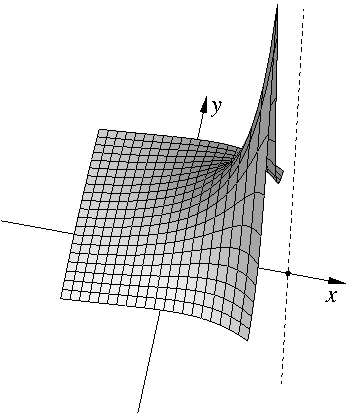
\includegraphics{figures/real1over1mz}
\qquad
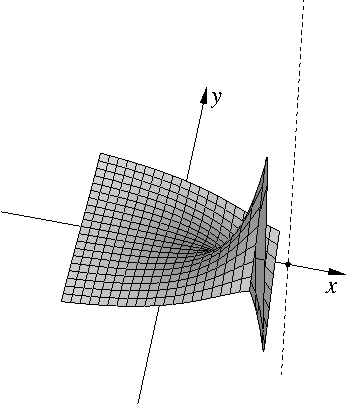
\includegraphics{figures/imag1over1mz}
\caption{Graphs of the real and imaginary parts of $z=x+iy \mapsto \frac{1}{1-z}$
in the square $[-0.8,0.8]^2$.\label{fig:1over1mz}}
\end{myfigureht}

\subsection{Convergence of power series}

We proved several results for power series of a real variable in
\volIref{\S2.6 of volume I}.   For the most part the convergence
properties of power series deal with the series
$\sum \sabs{c_k} \, \sabs{z-a}^k$ and so we have already proved many results about complex power
series.  In particular, we compute the so-called
\emph{\myindex{radius of convergence}} of a power series.

\begin{prop}
Let $\sum_{n=0}^\infty c_n {(z-a)}^n$ be a power series.
If the series is convergent, then either it converges at
all $z \in \C$, or
there exists a number $\rho$, such that
the series converges absolutely on $B(z,\rho)$
and diverges when $\sabs{z-a} > \rho$.
\end{prop}

\begin{proof}
We use the real version of this proposition,
\volIref{Proposition 2.6.10 in volume I}.
Let
\begin{equation*}
R := \limsup_{n\to\infty} \sqrt[n]{\sabs{c_n}} .
\end{equation*}
If $R = 0$, then
$\sum_{n=0}^\infty \sabs{c_n} \, \sabs{(z-a)}^n$ converges for all $z$.
If $R = \infty$, then
$\sum_{n=0}^\infty \sabs{c_n} \, \sabs{(z-a)}^n$ converges only at $z=a$.
Otherwise, let $\rho := \nicefrac{1}{R}$ and
$\sum_{n=0}^\infty \sabs{c_n} \, \sabs{(z-a)}^n$ converges when
$\sabs{z-a} < \rho$, and diverges (in fact the terms of the series
do not go to zero) when $\sabs{z-a} > \rho$.
The theorem follows.
\end{proof}

The number $\rho$ is called the \emph{\myindex{radius of convergence}}.
See \figureref{fig:radiusconvcomplex}.
We define $\rho$ even in cases when $R=0$ or $R= \infty$.  If $R=0$, we say
$\rho := \infty$ and if $R=\infty$ we say $\rho:=0$.
The radius of convergence gives us a disk around $a$ where the series converges.  A power series
is convergent if $\rho > 0$.
\begin{myfigureht}
\subimport*{figures/}{radiusconvcomplex.pdf_t}
\caption{Radius of convergence.\label{fig:radiusconvcomplex}}
\end{myfigureht}

It is trivial to see that if $\sum c_n {(z-a)}^n$ converges
for some $z$, then
\begin{equation*}
\sum c_n {(w-a)}^n
\end{equation*}
must converge absolutely whenever $\sabs{w-a} < \sabs{z-a}$.
Conversely if the series diverges at $z$, then it must diverge at $w$
whenever $\sabs{w-a} > \sabs{z-a}$.
This means that to show
that the radius of convergence is at least some number, we simply need to
show convergence at some point by any method we know.

\begin{example}
Let us list some series we already know:
\begin{align*}
& &
& \sum_{n=0}^\infty z^n
& & \text{has radius of convergence $1$.}
& &
\\
& &
& \sum_{n=0}^\infty \frac{1}{n!} z^n
& & \text{has radius of convergence $\infty$.}
& &
\\
& &
& \sum_{n=0}^\infty n^n z^n
& & \text{has radius of convergence $0$.}
& &
\end{align*}
\end{example}

Note the difference between $\frac{1}{1-z}$ and its power series.  Let us
expand $\frac{1}{1-z}$ as power series around any point $a \not= 1$.
Let $c = \frac{1}{1-a}$, then we can write
\begin{equation*}
\frac{1}{1-z} = 
\frac{c}{1-c(z-a)}
=
c
\sum_{n=0}^\infty c^{n} {(z-a)}^n
=
\sum_{n=0}^\infty \left( \frac{1}{{(1-a)}^{n+1}} \right) {(z-a)}^n .
\end{equation*}
Then notice that $\sum c^n {(z-a)}^n$ converges if and only if 
the power series on the right hand side converges and
\begin{equation*}
\limsup_{k\to\infty}
\sqrt[k]{c^k} = c
= \frac{1}{\sabs{1-a}} .
\end{equation*}
So radius of convergence of the power series is $\sabs{1-a}$, that is the
distance of $a$ from $1$.  In particular the function has a power series
representation around every $a$ not equal to 1 and so is analytic.
Notice that the domain of the function is bigger than the region
of convergence of any power series representing the function at any point.

It turns out that 
if a function has a power series representation converging to the function
on some ball,
then it has a representation at every point in the ball.  We will prove this
result later.

\subsection{Properties of analytic functions}

\begin{prop}
If
\begin{equation*}
f(z) := \sum c_n {(z-a)}^n
\end{equation*}
is convergent in $B(a,\rho)$ for some $\rho > 0$, then
$f \colon B(a,\rho) \to \C$ is continuous.
In particular, analytic functions are continuous.
\end{prop}

\begin{proof}
For any $z_0 \in B(a,\rho)$ pick $r < \rho$ such that $z_0 \in B(a,r)$.
If we show
that $f$ restricted to $B(a,r)$ is continuous then $f$ is continuous at
$z_0$.  This can be easily seen since any sequence converging to
$z_0$ has some tail that is completely in the open ball $B(a,r)$.  On $B(a,r)$ the
partial sums converge uniformly and so the limit is
continuous.
\end{proof}

Note that we can always apply an affine transformation $z \mapsto z+a$ which
converts the series to a series at the origin.  Therefore it is usually
sufficient to prove results about power series at the origin.
Therefore, from now on, let us assume $a=0$ for simplicity.

\medskip

In \volIref{Corollary 6.2.11 of volume I} we proved that we can
differentiate real power series term by term.  That is
we proved that if
\begin{equation*}
f(x) := \sum_{n=0}^\infty c_n x^n
\end{equation*}
converged in some interval around $0$, then we could differentiate
term by term and obtain a series
\begin{equation*}
f'(x) =
\sum_{n=1}^\infty n c_n {x}^{n-1}
=
\sum_{n=0}^\infty (n+1)c_{n+1} {x}^{n} 
\end{equation*}
with the same radius of convergence.
We only proved this theorem when $c_n$ were real, however writing
$c_n = a_n + i b_n$ we only need to apply the theorem to the real and
imaginary part as
\begin{equation*}
\sum_{n=0}^\infty c_n x^n
=
\sum_{n=0}^\infty a_n x^n
+
i
\sum_{n=0}^\infty b_n x^n .
\end{equation*}

By iterating this theorem we find that an
analytic function is infinitely differentiable:
\begin{equation*}
f^{(\ell)}(x) =
\sum_{n=\ell}^\infty n(n-1)\cdots(n-\ell+1)c_k {(x-a)}^{n-\ell}
=
\sum_{n=0}^\infty (n+\ell)(n+\ell-1)\cdots (n+1) c_{n+\ell} {(x-a)}^{n} .
\end{equation*}
In particular,
\begin{equation} \label{eq:formulaforpscoeffs}
f^{(\ell)}(a) = \ell! \, c_\ell .
\end{equation}
So the coefficients are determined by the derivatives of the
function.  In particular, once we have a function defined in
a neighborhood, the coefficients are unique:  If we have two power
series convergent in $(-\rho,\rho)$ such that for all $x \in (-\rho,\rho)$
\begin{equation*}
\sum_{n=0}^\infty c_n x^n
=
\sum_{n=0}^\infty c'_n x^n
\end{equation*}
then $c_n = c'_n$ for all $n$.

On the other hand, just because we have an infinitely differentiable
function doesn't mean that the numbers $c_n$ obtained by
$c_n = \frac{f^{(n)}(0)}{n!}$ give a convergent power series.  In fact,
there is a theorem, which we will not prove,
that given an arbitrary sequence $\{ c_n \}$, there exists an
infinitely differentiable function $f$ such that
$c_n = \frac{f^{(n)}(0)}{n!}$.  Finally, even if the obtained series
converges it may not converge to the function we started with.
For a simpler example,
see \volIref{Exercise 5.4.11 in volume I}.  That is the
function
\begin{equation*}
f(x) :=
\begin{cases}
e^{-1/x} & \text{if $x > 0$,}\\
0 & \text{if $x \leq 0$,}
\end{cases}
\end{equation*}
is infinitely differentiable, and all derivatives at the origin are zero, so
its series at the origin would be just the zero series, and while that
series converges, it does not converge to $f$ for $x > 0$.

\subsection{Power series as analytic functions}

We need a theorem on swapping limits of series, that is, 
Fubini's theorem for sums.

\begin{thm}[\myindex{Fubini for sums}] \label{thm:fubiniforsums}
Let $\{ a_{ij} \}_{i=1,j=1}^\infty$ be a double
sequence of complex numbers and suppose that for every $i$ the series
\begin{equation*}
\sum_{j=1}^\infty \sabs{a_{ij}} \qquad \text{converges}
\end{equation*}
and furthermore that
\begin{equation*}
\sum_{i=1}^\infty \left( \sum_{j=1}^\infty \sabs{a_{ij}} \right)
\qquad \text{converges}.
\end{equation*}
Then
\begin{equation*}
\sum_{i=1}^\infty \left( \sum_{j=1}^\infty a_{ij} \right)
=
\sum_{j=1}^\infty \left( \sum_{i=1}^\infty a_{ij} \right) ,
\end{equation*}
where all the series involved converge.
\end{thm}

\begin{proof}
Let $E$ be the set $\{ \nicefrac{1}{n} : n \in \N \} \cup \{ 0 \}$,
and treat it as a metric space with the metric inherited from $\R$.
Define the sequence of functions $f_i \colon E \to \C$
by
\begin{equation*}
f_i(\nicefrac{1}{n}) := \sum_{j=1}^n a_{ij}
\qquad
f_i(0) := \sum_{j=1}^\infty a_{ij}
\end{equation*}
As the series converge we get that each $f_i$ is continuous at $0$
(since 0 is the only cluster point, they are continuous everywhere, but
we don't need that).
For all $x \in E$ we have
\begin{equation*}
\sabs{f_i(x)} \leq \sum_{j=1}^\infty \sabs{a_{ij}}
\end{equation*}
By knowing that $\sum_i \sum_j \sabs{a_{ij}}$ converges (does not depend on
$x$), we know that for any $x \in E$
\begin{equation*}
\sum_{i=1}^n f_i(x)
\end{equation*}
converges uniformly.  So define
\begin{equation*}
g(x) := \sum_{i=1}^\infty f_i(x) ,
\end{equation*}
which is therefore a continuous function at $0$.
So
\begin{equation*}
\begin{split}
\sum_{i=1}^\infty \left( \sum_{j=1}^\infty a_{ij} \right)
& =
\sum_{i=1}^\infty f_i(0)
= g(0)
= \lim_{n\to\infty} g(\nicefrac{1}{n}) \\
&= 
\lim_{n\to\infty}\sum_{i=1}^\infty f_i(\nicefrac{1}{n})
= 
\lim_{n\to\infty}\sum_{i=1}^\infty \sum_{j=1}^n a_{ij} \\
&= 
\lim_{n\to\infty}\sum_{j=1}^n \sum_{i=1}^\infty a_{ij}
= 
\sum_{j=1}^\infty \left( \sum_{i=1}^\infty a_{ij} \right) . \qedhere
\end{split}
\end{equation*}
\end{proof}

Now we prove that once we have a series converging to a function
in some interval, we can expand the function around any point.

\begin{thm}[Taylor's theorem for real-analytic functions]
\label{thm:tayloranal}
Let
\begin{equation*}
f(x) := \sum_{k=0}^\infty a_k x^k
\end{equation*}
be a power series converging in $(-\rho,\rho)$ for some $\rho > 0$.  Given any $a \in
(-\rho,\rho)$, we obtain
for $x$ such that $\sabs{x-a} < \rho-\sabs{a}$ that
\begin{equation*}
f(x) =
\sum_{k=0}^\infty \frac{f^{(k)}(a)}{k!} {(x-a)}^{k} .
\end{equation*}
\end{thm}

The power series at $a$ could of course converge in a larger interval, but
the one above is guaranteed.  It is the largest symmetric interval about
$a$ that fits in $(-\rho,\rho)$.

\begin{proof}
Write
\begin{equation*}
\begin{split}
f(x) &= \sum_{k=0}^\infty a_k {\bigl((x-a)+a\bigr)}^k \\
&= \sum_{k=0}^\infty a_k \sum_{m=0}^k \binom{k}{m} a^{k-m} {(x-a)}^m %\\
%&= \sum_{m=0}^\infty \left( \sum_{k=0}^\infty a_k \sum_{m=0}^k \binom{k}{m}
%a^{k-m} \right) {(x-a)}^m
\end{split}
\end{equation*}
We define $c_{k,m} := a_k \binom{k}{m} a^{k-m}$ if $m \leq k$ and $0$ if $m >
k$, then we have
\begin{equation} \label{eq:tsproof}
f(x) = \sum_{k=0}^\infty \, \sum_{m=0}^\infty c_{k,m} {(x-a)}^m
\end{equation}
If we show that the double sum converges absolutely as in \thmref{thm:fubiniforsums} we
are done.  We can swap the order of the summations and obtain the desired
coefficients.
\begin{equation*}
\begin{split}
\sum_{k=0}^\infty \, \sum_{m=0}^\infty \abs{ c_{k,m} {(x-a)}^m}
& = \sum_{k=0}^\infty \, \sum_{m=0}^k \abs{ a_k \binom{k}{m} a^{k-m} {(x-a)}^m }
\\
& = \sum_{k=0}^\infty \sabs{a_k} \sum_{m=0}^k \binom{k}{m} \sabs{a}^{k-m}
{\sabs{x-a}}^m  \\
& = \sum_{k=0}^\infty \sabs{a_k} {\bigl(\sabs{x-a}+\sabs{a}\bigr)}^k
\end{split}
\end{equation*}
and this converges as long as 
$(\sabs{x-a}+\sabs{a}) < \rho$ or in other words if
$\sabs{x-a} < \rho-\sabs{a}$.

Now we swap the order of summation in \eqref{eq:tsproof}, and 
the following converges when $\sabs{x-a} < \rho-\sabs{a}$:
\begin{equation*}
f(x) =
\sum_{k=0}^\infty \, \sum_{m=0}^\infty c_{k,m} {(x-a)}^m
=
\sum_{m=0}^\infty
\left( \sum_{k=0}^\infty
c_{k,m} \right) {(x-a)}^m .
\end{equation*}
And we are done.  The formula in terms of derivatives at $a$ follows by
differentiating the series to obtain \eqref{eq:formulaforpscoeffs}.
\end{proof}

Note that if a series converges for $x \in (-\rho,\rho)$ it also converges
for all complex numbers in $B(0,\rho)$.
We have the following corollary.

\begin{cor}
If $\sum c_k {(z-a)}^k$ converges to $f(z)$ in $B(a,\rho)$ and $b \in
B(a,\rho)$,
then there exists a power series
$\sum d_k {(z-b)}^k$ that converges to $f(z)$ in $B(b,\rho-\sabs{b-a})$.
\end{cor}

\begin{proof}
Without loss of generality assume that $a=0$.  We can also rotate to assume that $b$ is real, but
since that is harder to picture, let us do it explicitly.
Let $\alpha = \frac{\widebar{b}}{\sabs{b}}$.
Notice that
\begin{equation*}
\abs{\nicefrac{1}{\alpha}} = \sabs{\alpha} %= \abs{\frac{\widebar{b}}{\sabs{b}}}
%=
%\sqrt{
%\frac{\widebar{b}}{\sabs{b}}
%\frac{b}{\sabs{b}}
%}
= 1 .
\end{equation*}
Therefore the series converges in $B(0,\rho)$
if we replace $z$ with $\nicefrac{z}{\alpha}$.
We apply \thmref{thm:tayloranal} at $\sabs{b}$ and get that a series that converges
to $f(\nicefrac{z}{\alpha})$ on $B(\sabs{b},\rho-\sabs{b})$.
That is, there are some coefficients $a_k$ such that
\begin{equation*}
f(\nicefrac{z}{\alpha}) =
\sum_{k=0}^\infty a_k {\bigl(z - \sabs{b}\bigr)}^k .
\end{equation*}
Notice that $\alpha b = \sabs{b}$.
\begin{equation*}
f(z) = f(\nicefrac{\alpha z}{\alpha}) =
\sum_{k=0}^\infty a_k {(\alpha z - \sabs{b})}^k 
=
\sum_{k=0}^\infty a_k\alpha^k {\bigl(z - \nicefrac{\sabs{b}}{\alpha}\bigr)}^k
=
\sum_{k=0}^\infty a_k\alpha^k {(z - b)}^k ,
\end{equation*}
and this converges for all $z$ such that
$\bigl\lvert \alpha z-\sabs{b}\bigr\rvert < \rho-\sabs{b}$
or $\sabs{z - b} < \rho-\sabs{b}$, which is the conclusion of the theorem.
\end{proof}

We proved above that a convergent power series is an
analytic function where it converges.  We have also shown before that
$\frac{1}{1-z}$ is analytic outside of $z=1$.

Note that just because a real analytic function is analytic on the
real line it doesn't necessarily mean that it has a power series
representation that converges everywhere.  For example, the function
\begin{equation*}
f(x) = \frac{1}{1+x^2}
\end{equation*}
happens to be real analytic.  It is pretty easy to show this (exercise).  A power
series around the origin converging to $f$ can have a radius of convergence at most $1$,
actually it does happen to be exactly 1.  Can you see why? (exercise).

\subsection{Identity theorem for analytic functions}

\begin{lemma}
Suppose $f(z) = \sum a_k z^k$ is a convergent power series and
$\{ z_n \}$ is a sequence of nonzero complex numbers converging to 0,
such that $f(z_n) = 0$ for all $n$.  Then $a_k = 0$ for every $k$.
\end{lemma}

\begin{proof}
By continuity we know $f(0) = 0$ so $a_0 = 0$.
Suppose there exists some nonzero $a_k$.
Let $m$ be the smallest $m$ such that $a_m \not= 0$.  Then
\begin{equation*}
f(z) = \sum_{k=m}^\infty a_k z^k = 
z^m \sum_{k=m}^\infty a_k z^{k-m} =
z^m \sum_{k=0}^\infty a_{k+m} z^{k} .
\end{equation*}
Write $g(z) = \sum_{k=0}^\infty a_{k+m} z^{k}$ (this series converges in
on the same set as $f$).  $g$ is continuous and $g(0) = a_m \not= 0$.  Thus
there exists some $\delta > 0$ such that $g(z) \not= 0$ for all $z \in
B(0,\delta)$.  As $f(z) = z^m g(z)$, then the only point in $B(0,\delta)$ where
$f(z) = 0$ is when $z=0$, but this contradicts the assumption
that $f(z_n) = 0$ for all $n$.
\end{proof}

Recall that in a metric space $X$, a \emph{cluster point}
(or sometimes \emph{limit point}) of a set
$E$ is a point $p \in X$ such that
$B(p,\epsilon) \setminus \{ p \}$ contains points of $E$
for all $\epsilon > 0$.

\begin{thm}[Identity theorem]
Let $U \subset \C$ be an open connected set.  If $f \colon U \to \C$
and $g \colon U \to \C$ are analytic functions that are
equal on a set $E \subset U$, and $E$ has a cluster point
in $U$, then $f(z) = g(z)$ for all $z \in U$.
\end{thm}

\begin{proof}
Without loss of generality suppose $E$ is the set of all points $z \in U$ such that
$g(z)=f(z)$.  Note that $E$ must be closed as $f$ and $g$ are continuous.

Suppose $E$ has a cluster point.  Without loss of generality assume that $0$ is the cluster point.  Near 0,
we have the expansions
\begin{equation*}
f(z) = \sum_{k=0}^\infty a_k {z}^k 
\qquad
\text{and}
\qquad
g(z) = \sum_{k=0}^\infty b_k {z}^k ,
\end{equation*}
which converge in some ball $B(0,\rho)$.  Therefore the series
\begin{equation*}
0 = f(z)-g(z) = 
\sum_{k=0}^\infty (a_k-b_k) z^k
\end{equation*}
converges in $B(0,\rho)$.  As $0$ is a cluster point of $E$, then there
is a sequence of nonzero points $\{ z_n \}$ such that
$f(z_n) -g(z_n) = 0$.  Therefore by the lemma above we have
that $a_k = b_k$ for all $k$.  And therefore $B(0,\rho) \subset E$.

This means that $E$ is open.  As $E$ is also closed, and $U$ is connected, we conclude that $E = U$.
\end{proof}

By restricting our attention to real $x$ we obtain the same
theorem for connected open subsets of $\R$, which are just open intervals.

\subsection{Exercises}

\begin{exercise}
Let $f(x) := \frac{1}{1+x^2}$.  Prove that the radius of convergence of
the power series for $f$ at the origin is 1.
\end{exercise}


\begin{exercise}
Suppose $f \colon \C \to \C$ is an analytic function.  Show that for each
$n$, there are at most finitely many zeros of $f$ in $B(0,n)$, that is
$f^{-1}(0) \cap B(0,n)$ is finite for each $n$.
\end{exercise}

\begin{exercise}
Suppose $U \subset \C$ is a connected open set, $0 \in U$, and $f \colon U
\to \C$ is an analytic function.  Treating $f$ as a function of a real $x$
at the origin, suppose $f^{(n)}(0) = 0$ for all $n$.  Show that $f(z) = 0$
for all $z \in U$.
\end{exercise}

\begin{exercise}
Suppose $U \subset \C$ is a connected open set, $0 \in U$, and $f \colon U
\to \C$ is an analytic function.  Let $h(x) := f(x)$ and $g(y) := -i \, f(iy)$.
Show that $h$ and $g$ are infinitely differentiable at the origin and
$h'(0) = g'(0)$.
\end{exercise}

\begin{exercise}
Suppose $f(z) := \sum c_n z^n$ with a radius of convergence 1.  Suppose $f(0)
= 0$.  Show that there exists a $k \in \N$ and a convergent
power series $g(z) := \sum d_n z^k$ with radius of convergence 1
such that $f(z) = z^k g(z)$ for all $z \in B(0,1)$.
\end{exercise}

%%%%%%%%%%%%%%%%%%%%%%%%%%%%%%%%%%%%%%%%%%%%%%%%%%%%%%%%%%%%%%%%%%%%%%%%%%%%%%

\sectionnewpage
\section{Fundamental theorem of algebra}
\label{sec:fundalgeb}

\sectionnotes{half a lecture}

In this section we study first the local behaviour of polynomials
and the growth of polynomials as $z$ goes to infinity.  As an application
we prove the fundamental theorem of algebra: any polynomial
has a complex root.

\begin{lemma} \label{lemma:polyalwaysgetssmaller}
Let $p(z)$ be complex polynomial.  If $p(z_0) \not= 0$, then there
exist $w \in \C$ such that $\sabs{p(w)} < \sabs{p(z_0)}$.  In fact,
we can pick $w$ to be arbitrarily close to $z_0$.
\end{lemma}

\begin{proof}
Without loss of generality assume that $z_0 = 0$ and $p(0) = 1$.  Then write
\begin{equation*}
p(z) = 1+a_kz^k + a_{k+1}z^{k+1} + \cdots + a_d z^d
\end{equation*}
where $a_k \not= 0$.  Pick $t$ such that $a_k e^{ikt} = -\sabs{a_k}$ which
we can do by the discussion on trigonometric functions.  Then for
any $r > 0$ small enough such that
$1-r^k \sabs{a_k} > 0$ we have
\begin{equation*}
p(r e^{it}) =
1-r^k \sabs{a_k} + r^{k+1}a_{k+1}e^{i(k+1)t} + \cdots + r^{d}a_{d}e^{idt} .
\end{equation*}
So
\begin{equation*}
\begin{split}
\abs{
p(r e^{it}) } - \abs{
r^{k+1}a_{k+1}e^{i(k+1)t} + \cdots + r^{d}a_{d}e^{idt}
}
& \leq
\abs{
p(r e^{it}) 
- r^{k+1}a_{k+1}e^{i(k+1)t} - \cdots - r^{d}a_{d}e^{idt}
}
\\
& =
\abs{
1-r^k \sabs{a_k}
}
=
1-r^k \sabs{a_k} .
\end{split}
\end{equation*}
In other words
\begin{equation*}
\abs{
p(r e^{it}) }
\leq
1-r^k \left( \sabs{a_k}
-
r
\abs{
a_{k+1}e^{i(k+1)t} + \cdots + r^{d-k-1}a_{d}e^{idt}
}
\right)
\end{equation*}
For a small enough $r$ the expression the parentheses is positive
as $\sabs{a_k} > 0$.  And then $\abs{p(re^{it})} < 1 = p(0)$.
\end{proof}

\begin{remark}
The above lemma holds essentially with an unchanged proof for (complex) analytic
functions.  A proof of this generalization is left as an exercise to the reader.
What the lemma
says is that the only minima the modulus of analytic functions (polynomials)
has are precisely at the zeros.
\end{remark}

\begin{remark}
The lemma does not hold if we restrict to real numbers.  For
example, $x^2+1$ has a minimum at $x=0$, but no zero there.  The thing is that
there is a $w$ arbitrarily close to $0$ such that $\sabs{w^2+1} < 1$, but this
$w$ is necessarily not real.  Letting $w = i\epsilon$ for small
$\epsilon > 0$ works.
\end{remark}

The moral of the story is that if $p(0) = 1$, then very close to 0, the
polynomial
looks like $1+az^k$ and this has no minimum at the origin.  All the higher
powers of $z$ are too small to make a difference.

\begin{lemma}
Let $p(z)$ be complex polynomial.  Then for any $M$ there exists
an $R$ such that if $\sabs{z} \geq R$ then $\sabs{p(z)} \geq M$.
\end{lemma}

\begin{proof}
Write $p(z) = a_0 + a_1 z + \cdots + a_d z^d$ and suppose that
$a_d \not= 0$.
Suppose $\sabs{z} \geq R$ (so also $\sabs{z}^{-1} \leq R^{-1}$).
We estimate:
\begin{equation*}
\begin{split}
\sabs{p(z)}
& \geq
\sabs{a_d z^d} -
\sabs{a_0} - \sabs{a_1 z} - \cdots - \sabs{a_{d-1} z^{d-1} }
\\
& =
\sabs{z}^d \bigl(
\sabs{a_d} -
\sabs{a_0} \sabs{z}^{-d} -
\sabs{a_1} \sabs{z}^{-d+1} - \cdots - \sabs{a_{d-1}} \sabs{z}^{-1}
\bigr)
\\
& \geq
R^d \bigl(\sabs{a_d} -
\sabs{a_0}R^{-d} - \sabs{a_1}R^{1-d} - \cdots - \sabs{a_{d-1}}R^{-1} \bigr)
.
\end{split}
\end{equation*}
Then the expression in parentheses is eventually positive for large enough
$R$.  In particular, for large enough $R$ we get that it is greater than
$\frac{\sabs{a_d}}{2}$ and so
\begin{equation*}
\sabs{p(z)}
\geq
R^d \frac{\sabs{a_d}}{2} .
\end{equation*}
Therefore,
we can pick $R$ large enough to be bigger than a given $M$.
\end{proof}

The above lemma does \emph{not} generalize to analytic
functions, even those defined in all of $\C$.  The function
$\cos(z)$ is an obvious counterexample.
Note that we had to look
at the term with the largest degree, and we only have such a term for
a polynomial.  In fact, something that we will not prove is that
an analytic function defined on all of $\C$ satisfying the conclusion
of the lemma
must be a polynomial.

The moral of the story here is that for very large $\sabs{z}$ (far away from
the origin) a polynomial of degree $d$ really looks like a constant multiple
of $z^d$.

\begin{thm}[Fundamental theorem of algebra]
Let $p(z)$ be complex polynomial, then there exists a $z_0 \in \C$
such that $p(z_0) = 0$.
\end{thm}

\begin{proof}
Let $\mu := \inf \bigl\{ \sabs{p(z)} : z \in \C \bigr\}$.  Find an $R$ such that
for all $z$ with $\sabs{z} \geq R$ we have $\sabs{p(z)} \geq \mu+1$.
Therefore, any $z$ with $\sabs{p(z)}$ close to $\mu$ must be in the
closed ball $C(0,R) = \bigl\{ z \in \C : \sabs{z} \leq R \bigr\}$.  As $\sabs{p(z)}$
is a continuous real-valued function, it achieves its minimum
on the compact set $C(0,R)$ (closed and bounded) and this minimum must
be $\mu$.  So there is a $z_0 \in C(0,R)$ such that $\sabs{p(z_0)} = \mu$.
As that is a minimum of $\sabs{p(z)}$ on $\C$, then by a lemma above we have
that $\sabs{p(z_0)} = 0$.
\end{proof}

The theorem doesn't generalize to analytic functions either.  For example
$e^{z}$ is an analytic function on $\C$ with no zeros.

\subsection{Exercises}

\begin{exercise} \label{exercise:minprinciple}
Prove \lemmaref{lemma:polyalwaysgetssmaller} for an analytic function.  That
is, suppose that $p(z)$ is not a polynomial but a power series around $z_0$.
\end{exercise}

\begin{exercise}
Use \exerciseref{exercise:minprinciple} to prove the \emph{\myindex{maximum
principle for analytic functions}}: \emph{If $U \subset \C$ is open and connected,
$f \colon U \to \C$ is analytic, and $\sabs{f(z)}$ attains a relative
maximum at $z_0 \in U$.  Then $f$ is constant.}
\end{exercise}

%%%%%%%%%%%%%%%%%%%%%%%%%%%%%%%%%%%%%%%%%%%%%%%%%%%%%%%%%%%%%%%%%%%%%%%%%%%%%%

\sectionnewpage
\section{The complex exponential and the trigonometric functions}
\label{sec:complexexp}

\sectionnotes{1 lecture}

\subsection{The complex exponential}

Define
\begin{equation*}
E(z) := \sum_{n=0}^\infty \frac{1}{n!} z^n .
\end{equation*}
This series converges for all $z \in \C$.   We notice that $E(0) = 1$,
and that for $z=x \in \R$, $E(x) \in \R$.  Keeping $x$ real, we find
\begin{equation*}
\frac{d}{dx} \bigl( E(x) \bigr) = E(x)
\end{equation*}
by direct calculation.
In \volIref{\S5.4 of volume I (or by Picard's theorem)}, we proved that
the unique function satisfying $E' = E$ and
$E(0) = 1$ is the exponential.  In other words for $x \in \R$, $e^x = E(x)$.

For complex numbers $z$ we define
\begin{equation*}
e^z := E(z) = 
\sum_{k=0}^\infty \frac{1}{k!} z^k .
\end{equation*}
And on the real line the two definitions agree.

\begin{prop}
Let $z,w \in \C$ be complex numbers.  Then
\begin{equation*}
e^{z+w} = e^z e^w.
\end{equation*}
\end{prop}

\begin{proof}
We know
$e^{x+y} = e^x e^y$ is true for
real numbers $x$ and $y$.

Now for any fixed $y \in \R$, we get by the
identity theorem (since the real numbers have a cluster point in $\C$) that
$e^{z+y} = e^ze^y$ for all $z \in \C$.  Fixing an arbitrary $z \in \C$
and we get
$e^{z+y} = e^ze^y$ for all $y \in \R$, and hence again by identity theorem we obtain
$e^{z+w} = e^z e^w$
for all $z,w \in \C$.
\end{proof}

\subsection{Trigonometric functions and $\pi$}

We can now finally define \emph{\myindex{sine}} and \emph{\myindex{cosine}}
by the equation
\begin{equation*}
e^{x+iy} = e^x \bigl( \cos(y) + i \sin(y) \bigr) .
\end{equation*}
In fact, we define sine and cosine for all complex $z$:
\begin{equation*}
\cos(z) := \frac{e^{iz} + e^{-iz}}{2}
\qquad\text{and}\qquad
\sin(z) := \frac{e^{iz} - e^{-iz}}{2i} .
\end{equation*}
Immediately we obtain the so called \emph{\myindex{Euler's formula}}:
\begin{equation*}
e^{iz} = \cos(z) + i\sin(z) .
\end{equation*}
From the definition of $e^z$ we notice that
$\overline{(e^z)} = e^{\widebar{z}}$ and so
if $x$ is real then
\begin{equation*}
\overline{(e^{ix})} = e^{-ix} .
\end{equation*}
Therefore when $x$ is real then we note that from the definition
\begin{equation*}
\cos(x) = \Re (e^{ix})
\qquad\text{and}\qquad
\sin(x) = \Im (e^{ix}) .
\end{equation*}
In other words, sine and cosine are real-valued when we plug in real $x$.

Also direct from the definition is that $\cos(-z) = \cos(z)$ and
$\sin(z) = -\sin(-z)$ for all $z \in \C$.

We will prove that this definition has the geometric properties we usually
associate with sin and cos.  Let $x$ be real and compute
\begin{equation*}
1 =  e^{ix} e^{-ix} = \sabs{e^{ix}}^2 = {\bigl( \cos(x) \bigr)}^2 + {\bigl( \sin(x) \bigr)}^2 .
\end{equation*}
We see that $e^{ix}$ is unimodular, the values lie on the unit circle.  By
noting that a square is always positive we notice that
\begin{equation*}
{\bigl(\sin(x)\bigr)}^2 = 1-{\bigl(\cos(x)\bigr)}^2 \leq 1
\end{equation*}
so $\sabs{\sin(x)} \leq 1$ and similarly we show
$\sabs{\cos(x)} \leq 1$.  A fact we have often used in examples.

From the definition we get that $\cos(0) = 1$ and $\sin(0) = 0$.  By direct
computation (left to reader) from the definition we also obtain:
\begin{equation*}
\cos(z) = \sum_{k=0}^\infty \frac{{(-1)}^k}{(2k)!} z^{2k} ,
\qquad
\sin(z) = \sum_{k=0}^\infty \frac{{(-1)}^k}{(2k+1)!} z^{2k+1} .
\end{equation*}

Again by direct calculation (again left to reader) we obtain
for real $x$
\begin{equation*}
\frac{d}{dx} \bigl( \cos(x) \bigr) = -\sin(x)
\qquad \text{and} \qquad
\frac{d}{dx} \bigl( \sin(x) \bigr) = \cos(x) .
\end{equation*}

Another fact that we have often used in examples was that $\sin(x) \leq x$
for $x \geq 0$.  Let us look at
$f(x) = x-\sin(x)$ and differentiate:
\begin{equation*}
f'(x) = \frac{d}{dx} \bigl( x - \sin(x) \bigr)
=
1 -\cos(x) \geq 0 ,
\end{equation*}
for all $x$ as $\sabs{\cos(x)} \leq 1$.
So $f$ is nondecreasing and
furthermore $f(0) = 0$.  So $f$ must be nonnegative when $x \geq 0$, which is
precisely what we wanted to prove.

We claim there exists a positive $x$ such that $\cos(x) = 0$.
As $\cos(0) = 1 > 0$, then cosine is definitely positive at least
for some $x$ near 0.
Suppose that on $[0,y)$ we have $\cos(x) > 0$, then $\sin(x)$ is strictly
increasing on $[0,y)$ and as $\sin(0) = 0$, then
$\sin(x) > 0$ for $x \in (0,y)$.  Take $a \in (0,y)$.  Then
for some $c \in (a,y)$
\begin{equation*}
2 \geq \cos(a)-\cos(y) = \sin(c)(y-a) \geq \sin(a)(y-a) .
\end{equation*}
As $a > 0$, then $\sin(a) > 0$ and so
\begin{equation*}
y \leq \frac{2}{\sin(a)} + a
\end{equation*}
Hence there is some largest $y$ such that $\cos(x) > 0$ in $[0,y)$.  By
continuity, for that $y$,
$\cos(y) = 0$.
In fact, $y$ is the
smallest positive $y$ such that $\cos(y) = 0$.  We can now define
\begin{equation*}
\pi := 2y .
\end{equation*}

And we obtain that $\cos(\frac{\pi}{2}) = 0$ and so
${\bigl(\sin(\frac{\pi}{2})\bigr)}^2 = 1$.
As $\sin$ was positive on $(0,y)$ we have
$\sin(\frac{\pi}{2}) = 1$.
Hence
\begin{equation*}
e^{i \pi /2} = i ,
\end{equation*}
and by the addition formula we get
\begin{equation*}
e^{i \pi} = -1 ,
\qquad 
e^{i 2\pi} = 1 .
\end{equation*}
So $e^{i2\pi} = 1 = e^0$.  The addition formula now says
that
\begin{equation*}
e^{z+i2\pi} = e^z
\end{equation*}
for all $z \in \C$.  Therefore, we also obtain that
\begin{equation*}
\cos(z+2\pi) = \cos(z)
\qquad\text{and}\qquad
\sin(z+2\pi) = \sin(z) .
\end{equation*}
So $\sin$ and $\cos$ are $2\pi$-periodic.
We claim that $\sin$ and $\cos$ are not periodic with a smaller period.  It
would be enough to show that if $e^{ix} = 1$ for the
smallest positive $x$, then
$x = 2\pi$.
Well let $x$ be the smallest positive $x$ such that
$e^{ix} = 1$.
Of course, $x \leq 2\pi$.
Then by the addition formula
\begin{equation*}
{\bigl(e^{ix/4}\bigr)}^4 = 1 .
\end{equation*}
If $e^{ix/4} = a+ib$, then
\begin{equation*}
{(a+ib)}^4
=a^4-6a^2b^2+b^4 + i\bigl(4ab(a^2-b^2)\bigr)
=1 .
\end{equation*}
As $\nicefrac{x}{4} \leq \nicefrac{\pi}{2}$, then $a = \cos(\nicefrac{x}{4}) \geq 0$ and
$0 < b = \sin(\nicefrac{x}{4})$.  Then either $a = 0$, in which case
$\nicefrac{x}{4} = \nicefrac{\pi}{2}$ or $a^2 = b^2$.  But if $a^2=b^2$, then
$a^4-6a^2b^2+b^4 = -4a^4 < 0$ and in particular not equal to 1.
Therefore $a=0$ in which case $\nicefrac{x}{4} = \nicefrac{\pi}{2}$.

Therefore $2\pi$ is the smallest period we could choose for $e^{ix}$
and hence $\cos$ and $\sin$.

Finally we also wish to show that $e^{ix}$ is 1-to-1 and onto
from the set $[0,2\pi)$ to the set of $z \in \C$ such that
$\sabs{z} = 1$.  First suppose that $e^{ix} = e^{iy}$ and assume that
$x > y$ then
$e^{i(x-y)} = 1$, which means that $x-y$ is a multiple of $2\pi$ and hence
only one of them can live in $[0,2\pi)$.
To show onto, pick $(a,b) \in \R^2$ such that $a^2+b^2 = 1$.
If $a,b \geq 0$, then there must exist an $x \in [0,\nicefrac{\pi}{2}]$ such that
$\cos(x) = a$, and hence $b^2 = \bigl(\sin(x)\bigr)^2$ and since
$b$ and $\sin(x)$ are positive we have $b = \sin(x)$.
Note that since $-\sin(x)$ is the derivative of $\cos(x)$
and $\cos(-x) = \cos(x)$ then $\sin(x) < 0$ for $x \in [\nicefrac{-\pi}{2},0)$.
Then using the same reasoning we obtain that if
if $a > 0$ and $b \leq 0$, we can find an $x \in [\nicefrac{-\pi}{2},0)$,
or in other words in $[\nicefrac{3\pi}{2},2\pi)$
As multiplying by $-1$ is the same as multiplying by $e^{i\pi}$ or
$e^{-i\pi}$
we can always assume that $a \geq 0$ (details left to student).

The arclength of a curve parametrized by $\gamma \colon [a,b] \to \C$ is given
by
\begin{equation*}
\int_a^b \sabs{\gamma'(t)} ~ dt .
\end{equation*}
We have that $e^{it}$ parametrizes the circle for $t$ in $[0,2\pi)$.
$\frac{d}{dt} \bigl( e^{it} \bigr) = ie^{it}$ and so the circumference of the
circle is
\begin{equation*}
\int_0^{2\pi} \sabs{i e^{it}}  ~  dt
=
\int_0^{2\pi} 1  ~  dt  = 2\pi .
\end{equation*}

More generally we notice that $e^{it}$ parametrizes the circle by arclength.
That is, $t$ measures the arclength, and hence a circle of radius 1 by
the angle in radians.  Hence the definitions of $\sin$ and $\cos$ we have
used above agree with the standard geometric definitions.

\subsection{Exercises}

\begin{exercise}
Derive the power series for $\sin(z)$ and $\cos(z)$ at the origin.
\end{exercise}

%%%%%%%%%%%%%%%%%%%%%%%%%%%%%%%%%%%%%%%%%%%%%%%%%%%%%%%%%%%%%%%%%%%%%%%%%%%%%%

\sectionnewpage
\section{Fourier series}
\label{sec:fourier}

\sectionnotes{3--4 lectures}

Fourier series is perhaps the most important of the series that we cover in
this book.  We have seen a few in examples before, but let us start
at the beginning.

\subsection{Trigonometric polynomials}

A \emph{\myindex{trigonometric polynomial}} is an expression of the form
\begin{equation*}
a_0 + \sum_{n=1}^N \bigl(a_n \cos(nx) + b_n \sin(nx) \bigr),
\end{equation*}
or equivalently, thanks to Euler's formula ($e^{i\theta} = \cos(\theta) + i
\sin(\theta)$):
\begin{equation*}
\sum_{n=-N}^N c_n e^{inx} .
\end{equation*}
The second form is usually more convenient.  Note that if
$\sabs{z}=1$ we can write $z = e^{ix}$, and so
\begin{equation*}
\sum_{n=-N}^N c_n e^{inx} = 
\sum_{n=-N}^N c_n z^n ,
\end{equation*}
so a trigonometric polynomial is really a rational function (do note that
we are allowing negative powers) evaluated on the unit circle.  There is
a wonderful connection between power series (actually Laurent series) and
Fourier series because of this observation,
but we will not investigate this further.

Notice that all the functions are $2\pi$-periodic and hence the trig
polynomials are also $2\pi$-periodic.
We could rescale $x$ to make the period different, but the theory is the
same, so we will stick with the above scale.
We compute that the antiderivative of $e^{inx}$ is $\frac{e^{inx}}{in}$ and
so
\begin{equation*}
\int_{-\pi}^\pi e^{inx} ~ dx =
\begin{cases}
2\pi & \text{if $n=0$,} \\
0 & \text{otherwise.}
\end{cases}
\end{equation*}
Let us take
\begin{equation*}
f(x) = \sum_{n=-N}^N c_n e^{inx} ,
\end{equation*}
and for $m=-N,\ldots,N$ compute
\begin{equation*}
\frac{1}{2\pi} \int_{-\pi}^\pi
f(x) e^{-imx} ~ dx
=
\frac{1}{2\pi} \int_{-\pi}^\pi
\left(\sum_{n=-N}^N c_n e^{i(n-m)x}\right) ~ dx
=
\sum_{n=-N}^N
c_n
\frac{1}{2\pi}
\int_{-\pi}^\pi
e^{i(n-m)x}
 ~ dx
=
c_m .
\end{equation*}
We therefore have a way of computing the coefficients $c_m$ by an integral
of $f$.  Of course if $\sabs{m} > N$ the integral is just 0.  We might as
well have included enough zero coefficients to make $\sabs{m} \leq N$.

\begin{prop}
A trigonometric polynomial
$f(x) = \sum_{n=-N}^N c_n e^{inx}$
is real-valued for real $x$ if
and only if $c_{-m} = \overline{c_m}$ for all $m=-N,\ldots,N$.
\end{prop}

\begin{proof}
If $f(x)$ is real-valued, that is $\overline{f(x)} = f(x)$, then
\begin{equation*}
\overline{c_m}
=
\overline{
\frac{1}{2\pi} \int_{-\pi}^\pi
f(x) e^{-imx} ~ dx
}
=
\frac{1}{2\pi} \int_{-\pi}^\pi
\overline{
f(x) e^{-imx} } ~ dx
=
\frac{1}{2\pi} \int_{-\pi}^\pi
f(x) e^{imx} ~ dx
= c_{-m} .
\end{equation*}
The complex conjugate goes inside the integral because the integral is
done on real and imaginary parts separately.  On the other hand if 
$c_{-m} = \overline{c_m}$, then we notice that
\begin{equation*}
\overline{c_{-m} e^{-imx}+ c_{m} e^{imx}}
=
\overline{c_{-m}} e^{imx}+ \overline{c_{m}} e^{-imx}
=
c_{m} e^{imx}+ c_{-m} e^{-imx} .
\end{equation*}
We also have that $c_0 = \overline{c_0}$.
So by pairing up the terms we obtain that $f$ has to be real-valued.
\end{proof}

In fact, the above could also follow from the linear independence of the
functions $e^{inx}$, which we can now prove.

\begin{prop}
If
\begin{equation*}
\sum_{n=-N}^N c_n e^{inx} = 0
\end{equation*}
for all $x \in \R$, then $c_n = 0$ for all $n$.
\end{prop}

\begin{proof}
Proof follows immediately from the integral formula for $c_n$.
\end{proof}

\subsection{Fourier series}

We now take limits.  We call the series
\begin{equation*}
\sum_{n=-\infty}^\infty c_n e^{inx}
\end{equation*}
the \emph{\myindex{Fourier series}}.  The numbers $c_n$
we call \emph{\myindex{Fourier coefficients}}.  We could also develop everything with
sines and cosines, but it is equivalent and slightly more messy.

Several questions arise.  What functions are expressible as 
Fourier series?  Obviously, they have to be $2\pi$-periodic, but not every
periodic function is expressible with the series.  Furthermore, if we do have
a Fourier series, where does it converge (if at all)?  Does it converge
absolutely?  Uniformly (and where)?  Also note that the series has two
limits.  When talking about Fourier series convergence, we often
talk about the following limit:
\begin{equation*}
\lim_{N\to\infty} 
\sum_{n=-N}^N c_n e^{inx} .
\end{equation*}
There are other ways we can sum the series that can get convergence in more
situations, but we refrain from discussing those.

For any function integrable on $[-\pi,\pi]$ we call the numbers
\begin{equation*}
c_n = 
\frac{1}{2\pi} \int_{-\pi}^\pi
f(x) e^{-inx} ~ dx
\end{equation*}
its Fourier coefficients.  Often these numbers are
written as $\hat{f}(n)$\footnote{If you have seen the Fourier transform,
the similarity is not just
coincidental, we are really taking a type of Fourier transform here}.
We then formally write down a Fourier series.
As you might imagine such a series might not even converge.
We write
\begin{equation*}
f(x) \sim
\sum_{n=-\infty}^\infty c_n e^{inx}
\end{equation*}
although the $\sim$ doesn't imply anything about the two sides being equal
in any way.  It is simply that we created a formal series using the formula
for the coefficients.

We have seen that the example Fourier series 
\begin{equation*}
\sum_{n=1}^\infty \frac{\sin(nx)}{n^2}
\end{equation*}
converges uniformly and hence is continuous.  This 
example can be extended to a more general criterion.

\begin{prop}
Let $\sum_{n=-\infty}^\infty c_n e^{inx}$ be a Fourier series,
and $C$, $\alpha > 1$ constants such that
\begin{equation*}
\sabs{c_n} \leq \frac{C}{\sabs{n}^\alpha}
\qquad \text{for all $n \in \Z \setminus \{ 0 \}$}.
\end{equation*}
Then the series converges (absolutely and uniformly) to a continuous function on $\R$.
\end{prop}

The proof is to apply the Weierstrass $M$-test (\thmref{thm:weiermtest}) and
the $p$-series test, to find that the series converges uniformly and hence
to a continuous function.
We can also take derivatives.

\begin{prop}
Let $\sum_{n=-\infty}^\infty c_n e^{inx}$ be a Fourier series,
and $C$, $\alpha > 2$ constants such that
\begin{equation*}
\sabs{c_n} \leq \frac{C}{\sabs{n}^\alpha}
\qquad \text{for all $n \in \Z \setminus \{ 0 \}$}.
\end{equation*}
Then the series converges to a continuously differentiable function on $\R$.
\end{prop}

The trick is to first notice that the series converges first to a continuous
function by the previous proposition, so in particular it converges at some
point.  Then differentiate the partial sums
\begin{equation*}
\sum_{n=-N}^{N}
i n c_n e^{inx}
\end{equation*}
and notice that 
\begin{equation*}
\sabs{in c_n} \leq \frac{C}{\sabs{n}^{\alpha-1}} .
\end{equation*}
The differentiated series converge uniformly by the $M$-test again.  Since
the derivatives converge uniformly, we find that the series converges 
to a continuously differentiable function.

In fact, by iterating the same reasoning we find that if
for some $C$ and $\alpha > k$ ($k \in \N$) we have
\begin{equation*}
\sabs{c_n} 
\leq \frac{C}{\sabs{n}^\alpha}
\end{equation*}
for all nonzero integers $n$.  Then 
the Fourier series converges to a $k$-times continuously differentiable
function.  Therefore, the faster the coefficients go to zero, the more
regular the limit is.

\subsection{Orthonormal systems}

Let us now investigate convergence of Fourier series from the other side.
Given properties of $f$, what can we say about the series.

Let us first prove some general results about so called
\emph{orthonormal systems}.
Let us fix an interval $[a,b]$.  We define an
\emph{\myindex{inner product}} for the space of functions.  We restrict our attention
to Riemann integrable functions since we do not have the Lebesgue
integral, which
would be the natural choice.  Let $f$ and $g$ be complex-valued 
Riemann integrable functions on $[a,b]$ and define the inner product
\begin{equation*}
\langle f , g \rangle :=
\int_a^b f(x) \overline{g(x)} ~ dx
\end{equation*}
If you have seen Hermitian inner products in linear algebra, this
is precisely such a product.  We have to put in the conjugate as we are
working with complex numbers.  We then have the ``size'', that is the
$L^2$ norm $\snorm{f}_2$ by (defining the square)
\begin{equation*}
\snorm{f}_2^2 :=
\langle f , f \rangle =
\int_a^b \sabs{f(x)}^2 ~ dx .
\end{equation*}

\begin{remark}
Notice the similarity to finite dimensions.  For $z = (z_1,z_2,\ldots,z_n) \in 
\C^n$ we define 
\begin{equation*}
\langle z , w \rangle :=
\sum_{k=1}^n z_k \overline{w_k}
\end{equation*}
and then the norm is (usually this is just denoted by $\snorm{z}$ rather than
$\snorm{z}_2$)
\begin{equation*}
\snorm{z}^2 = 
\langle z , z \rangle =
\sum_{k=1}^n \sabs{z_k}^2 .
\end{equation*}
This is just the euclidean distance to the origin in $\C^n$.
\end{remark}

Let us get back to function spaces.  We assume all functions are
Riemann integrable in the following.

\begin{defn}
Let $\{ \varphi_n \}$ be a sequence of integrable complex-valued
functions on $[a,b]$.  We say that this is an
\emph{\myindex{orthonormal system}} if
\begin{equation*}
\langle \varphi_n , \varphi_m \rangle
=
\int_a^b \varphi_n(x) \overline{\varphi_m(x)} ~ dx
= 
\begin{cases}
1 & \text{if $n=m$,} \\
0 & \text{otherwise.}
\end{cases}
\end{equation*}
Notice that the above says that $\snorm{\varphi_n}_2 = 1$ for all $n$.  If we
only require that 
$\langle \varphi_n , \varphi_m \rangle = 0$ for $m\not= n$ then
the system would be just an \emph{\myindex{orthogonal system}}.
\end{defn}

We have noticed above that for example
\begin{equation*}
\left\{ \frac{1}{\sqrt{2\pi}} \, e^{inx} \right\}
\end{equation*}
is an orthonormal system.  The factor out in front is to make the norm be 1.

Having an orthonormal system $\{ \varphi_n \}$ on $[a,b]$ and an integrable function $f$
on $[a,b]$, we can write
a Fourier series relative to $\{ \varphi_n \}$.  We let
\begin{equation*}
c_n =
\langle f , \varphi_n \rangle
=
\int_a^b f(x) \overline{\varphi_n(x)} ~ dx ,
\end{equation*}
and write
\begin{equation*}
f(x) \sim \sum_{n=1}^\infty c_n \varphi_n .
\end{equation*}

In other words, the series is
\begin{equation*}
\sum_{n=1}^\infty \langle f , \varphi_n \rangle \varphi_n(x) .
\end{equation*}
Notice the similarity to the expression for the orthogonal
projection of a vector onto a subspace from linear algebra.  We are
in fact doing just that, but in a space of functions.

\begin{thm} \label{thm:l2bestapprox}
Suppose $f$ is a Riemann integrable function on $[a,b]$.
Let $\{ \varphi_n \}$ be an orthonormal system on $[a,b]$ and
suppose
\begin{equation*}
f(x) \sim \sum_{n=1}^\infty c_n \varphi_n(x) .
\end{equation*}
If
\begin{equation*}
s_n (x) = \sum_{k=1}^n c_k \varphi_k(x)
\quad\text{and}\quad
t_n (x) = \sum_{k=1}^n d_k \varphi_k(x) .
\end{equation*}
for some other sequence $\{ d_k \}$, then
\begin{equation*}
\int_a^b \sabs{f(x)-s_n(x)}^2 ~ dx = \snorm{f-s_n}_2^2 \leq
\snorm{f-t_n}_2^2 = \int_a^b \sabs{f(x)-t_n(x)}^2 ~ dx .
\end{equation*}
with equality only if $d_k = c_k$ for all $k=1,2,\ldots,n$.
\end{thm}

In other words the partial sums of the Fourier series are the best approximation with respect to the
$L^2$ norm.

\begin{proof}
Let us write
\begin{equation*}
\int_a^b \sabs{f-t_n}^2
=
\int_a^b \sabs{f}^2
-
\int_a^b f \overline{t_n}
-
\int_a^b \overline{f} t_n
+
\int_a^b \sabs{t_n}^2 .
\end{equation*}
Now
\begin{equation*}
\int_a^b f \overline{t_n}
=
\int_a^b f \sum_{k=1}^n \overline{d_k} \overline{\varphi_k}
=
 \sum_{k=1}^n \overline{d_k} \int_a^b f \overline{\varphi_k}
=
 \sum_{k=1}^n \overline{d_k} c_k ,
\end{equation*}
and
\begin{equation*}
\int_a^b \sabs{t_n}^2
=
\int_a^b
\sum_{k=1}^n d_k \varphi_k
\sum_{j=1}^n \overline{d_j} \overline{\varphi_j}
=
\sum_{k=1}^n
\sum_{j=1}^n 
d_k
\overline{d_j} 
\int_a^b
\varphi_k
\overline{\varphi_j}
=
\sum_{k=1}^n
\sabs{d_k}^2 .
\end{equation*}
So
\begin{equation*}
\int_a^b \sabs{f-t_n}^2
=
\int_a^b \sabs{f}^2
-
\sum_{k=1}^n \overline{d_k} c_k
-
\sum_{k=1}^n d_k \overline{c_k}
+
\sum_{k=1}^n
\sabs{d_k}^2
=
\int_a^b \sabs{f}^2
-
\sum_{k=1}^n \sabs{c_k}^2
+
\sum_{k=1}^n
\sabs{d_k-c_k}^2 .
\end{equation*}
This is minimized precisely when $d_k = c_k$.
\end{proof}

When we do plug in $d_k = c_k$, then
\begin{equation*}
\int_a^b \sabs{f-s_n}^2
=
\int_a^b \sabs{f}^2
-
\sum_{k=1}^n \sabs{c_k}^2
\end{equation*}
and so
\begin{equation*}
\sum_{k=1}^n \sabs{c_k}^2
\leq
\int_a^b \sabs{f}^2
\end{equation*}
for all $n$.  Note that
\begin{equation*}
\sum_{k=1}^n \sabs{c_k}^2 = \snorm{s_n}_2^2
\end{equation*}
by the above calculation.
We can take a limit to obtain the so called
\emph{\myindex{Bessel's inequality}}.

\begin{thm}[Bessel's inequality] \label{thm:bessels}
Suppose $f$ is a Riemann integrable function on $[a,b]$.
Let $\{ \varphi_n \}$ be an orthonormal system on $[a,b]$ and
suppose
\begin{equation*}
f(x) \sim \sum_{n=1}^\infty c_n \varphi_n(x) .
\end{equation*}
Then
\begin{equation*}
\sum_{k=1}^\infty \sabs{c_k}^2
\leq
\int_a^b \sabs{f}^2
= \snorm{f}_2^2 .
\end{equation*}
\end{thm}

In particular (given that a Riemann integrable function satisfies
$\int_a^b \sabs{f}^2 < \infty$), we get that the series
converges and hence
\begin{equation*}
\lim_{k \to \infty} c_k = 0 .
\end{equation*}

\subsection{The Dirichlet kernel and approximate delta functions}

Let us return to the trigonometric Fourier series.  Here we note that the
system $\{ e^{inx} \}$ is orthogonal, but not orthonormal if we simply
integrate over $[-\pi,\pi]$.  We can also rescale the integral
and hence the inner product to make 
$\{ e^{inx} \}$ orthonormal.  That is, if we replace
\begin{equation*}
\int_a^b \qquad \text{with} \qquad
\frac{1}{2\pi} \int_{-\pi}^\pi
\end{equation*}
(we are just rescaling the $dx$ really)\footnote{%
In fact, this leads some authors to simplify matters by
making a tounge-in-cheek definition that $1=2\pi$.}
then everything works and we obtain that the system $\{ e^{inx} \}$
is orthonormal with respect to the inner product
\begin{equation*}
\langle f , g \rangle =
\frac{1}{2\pi} \int_{-\pi}^\pi f(x) \, \overline{g(x)} ~ dx .
\end{equation*}

So suppose we have an integrable function $f$ on $[-\pi,\pi]$.  In fact
suppose
that $f$ is a function defined on all of $\R$ and is $2\pi$ periodic.
Let
\begin{equation*}
c_n := 
\frac{1}{2\pi} \int_{-\pi}^\pi
f(x) e^{-inx} ~ dx .
\end{equation*}
Write
\begin{equation*}
f(x) \sim
\sum_{n=-\infty}^\infty c_n e^{inx} .
\end{equation*}
We define at the \emph{\myindex{symmetric partial sums}}
\begin{equation*}
s_N(x) = s_N(f;x) := 
\sum_{n=-N}^N c_n e^{inx} .
\end{equation*}
The inequality leading up to Bessel now reads:
\begin{equation*}
\frac{1}{2\pi} \int_{-\pi}^\pi
\sabs{s_N(x)}^2 ~ dx =
\sum_{n=-N}^N \sabs{c_n}^2
\leq
\frac{1}{2\pi} \int_{-\pi}^\pi
\sabs{f(x)}^2
~ dx .
\end{equation*}

Let us now define the \emph{\myindex{Dirichlet kernel}}
\begin{equation*}
D_N(x) := \sum_{n=-N}^N e^{inx} .
\end{equation*}
We claim that
\begin{equation*}
D_N(x) =
\sum_{n=-N}^N e^{inx}
=
\frac{\sin\bigl( (N+\nicefrac{1}{2})x \bigr)}{\sin(\nicefrac{x}{2})} ,
\end{equation*}
at least for $x$ such that $\sin(x/2) \not= 0$.  We know that the left hand
side is continuous and hence the right hand side extends continuously as well.
  %As we are only interested
%in this function on $[-\pi,\pi]$ we simply need to worry about $x=0$.
%We claim that when $x=0$ the right
%hand side is continuous (and its limit equals $D_N(x)$).
To show the claim
we use a familiar trick:
\begin{equation*}
(e^{ix}-1) D_N(x) = e^{i(N+1)x} - e^{-iNx} .
\end{equation*}
And multiply by $e^{-ix/2}$
\begin{equation*}
(e^{ix/2}-e^{-ix/2}) D_N(x) = e^{i(N+\nicefrac{1}{2})x} -
e^{-i(N+\nicefrac{1}{2})x} .
\end{equation*}
The claim follows.
%The claim follows at least when $\sin(x/2) \not=0$.
%Let us prove continuity at $0$.
%From the Taylor expansion of $\sin$ we know that
%$\sin(x) = x+x^2 g(x)$ for a continuous function $g(x)$.
%%Next we have the following useful
%%fact that follows from the taylor expansion of $\sin$.
%%We have that
%%inequalities for $x$ near the origin.
%%$$
%%\frac{\sabs{x}}{2} \leq \sabs{\sin(x)} \leq \sabs{x}
%%$$
%%The proof is left to the reader.  Using these inequalities we 
%Hence
%$$
%\frac{\sin\bigl( (N+\nicefrac{1}{2})x \bigr)}{\sin(\nicefrac{x}{2})}
%=
%\frac{(N+\nicefrac{1}{2})x  + {((N+\nicefrac{1}{2})x)}^2
%g((N+\nicefrac{1}{2})x)}{\nicefrac{x}{2}  + {(\nicefrac{x}{2})}^2
%g(\nicefrac{x}{2})}
%=
%\frac{(N+\nicefrac{1}{2})  + {(N+\nicefrac{1}{2})}^2x
%g((N+\nicefrac{1}{2})x)}{\nicefrac{1}{2}  + \nicefrac{x}{4}
%g(\nicefrac{x}{2})}
%$$
%Which is continuous at the origin.  Now when
%$x/2 = \pi k$, then
%$(N+\nicefrac{1}{2})x =
%(N+\nicefrac{1}{2})2\pi k
%=
%(2N+1)\pi k$, so the numerator of the expression also vanishes and same
%argument shows that the expression is continuous.
%Really you should be able to do these
%types of arguments from now on and I will only mention them in passing.

We expand the definition of $s_N$
\begin{equation*}
s_N(x) = 
\sum_{n=-N}^N \frac{1}{2\pi} \int_{-\pi}^\pi f(t) e^{-int}  ~  dt ~ e^{inx}
=
\frac{1}{2\pi} \int_{-\pi}^\pi f(t) \sum_{n=-N}^N e^{in(x-t)} ~ dt
=
\frac{1}{2\pi} \int_{-\pi}^\pi f(t) D_N(x-t) ~ dt .
\end{equation*}
Convolution strikes again!
As $D_N$ and $f$ are $2\pi$-periodic we can also change variables and write 
\begin{equation*}
s_N(x) = 
\frac{1}{2\pi} \int_{x-\pi}^{x+\pi} f(x-t) D_N(t) ~ dt
=
\frac{1}{2\pi} \int_{-\pi}^\pi f(x-t) D_N(t) ~ dt
\end{equation*}
See \figureref{fig:approxdeltas} for a plot of $D_N$ for $N=5$ and $N=20$.

\begin{myfigureht}
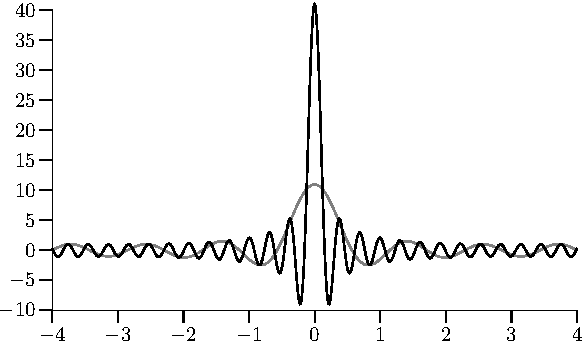
\includegraphics{figures/approxdeltas}
\caption{Plot of $D_N(x)$ for $N=5$ (gray) and $N=20$
(black).\label{fig:approxdeltas}}
\end{myfigureht}

The central peak will get taller and taller with $N$ being larger,
and the side peaks will stay small (but oscillate wildly).
We are convolving (again) with approximate delta functions,
although these have
all these oscillations away from zero which do not go away.  So we expect that
$s_N$ goes to $f$.  Things are not so simple, but under some conditions on
$f$, such a conclusion holds.  For this reason
people write
\begin{equation*}
\delta(x) \sim \sum_{n=\infty}^\infty e^{inx}
\end{equation*}
although we have not really defined the delta function (and it is not a
function), nor a Fourier series of whatever kind object it is.

\subsection{Localization}

\begin{thm}
Let $x$ be fixed and let $f$ be a $2\pi$-periodic function
Riemann integrable on $[-\pi,\pi]$.  Suppose
there exist $\delta > 0$ and $M$ such that
\begin{equation*}
\sabs{f(x+t)-f(x)} \leq M \sabs{t}
\end{equation*}
for all $t \in (-\delta,\delta)$, then
\begin{equation*}
\lim_{N \to \infty} s_N(f;x) = f(x) .
\end{equation*}
\end{thm}

In other words, if for example $f$ is differentiable at $x$
then we obtain convergence.  A useful consequence of
the result is
that if the function is continuous
piecewise smooth, then the Fourier series converges
(pointwise).   By continuous piecewise smooth we mean that $f$
is continuous and periodic so $f(-\pi) = f(\pi)$ and furthermore
that there are points $x_0 = -\pi < x_1 < \cdots < x_k = \pi$
such that $f$ restricted to $[x_j,x_{j+1}]$
is continuously differentiable (up to the endpoints) for all $j$.

\begin{proof}
We notice that for all $N$ we get
\begin{equation*}
\frac{1}{2\pi} \int_{-\pi}^\pi D_N = 1 .
\end{equation*}
Write
\begin{equation*}
\begin{split}
s_N(f;x)-f(x) & =
\frac{1}{2\pi} \int_{-\pi}^\pi f(x-t) D_N(t) ~ dt 
-
f(x)
\frac{1}{2\pi} \int_{-\pi}^\pi D_N(t) ~ dt
\\
& = 
\frac{1}{2\pi} \int_{-\pi}^\pi \bigl( f(x-t) - f(x) \bigr) D_N(t) ~ dt 
\\
& = 
\frac{1}{2\pi} \int_{-\pi}^\pi \frac{f(x-t) - f(x)}{\sin(\frac{t}{2})} \sin\bigl(
(N+\nicefrac{1}{2})t \bigr) ~ dt 
\end{split}
\end{equation*}
Now by the hypotheses we obtain that
for small nonzero $t$ we get
\begin{equation*}
\abs{ \frac{f(x-t) - f(x)}{\sin(\frac{t}{2})} }
\leq
\frac{M\sabs{t}}{\sabs{\sin(\frac{t}{2})}}
\end{equation*}
As $\sin(t) = t + h(t)$ where $\frac{h(t)}{t} \to 0$ as $t \to 0$,
we notice that
$\frac{M\sabs{t}}{\sabs{\sin(\frac{t}{2})}}$ is continuous at the origin
and hence 
$\frac{f(x-t) - f(x)}{\sin(\frac{t}{2})}$ must be bounded near the origin.
As $t=0$ is the only place on $[-\pi,\pi]$ where the denominator vanishes,
it is the only place where there could be a problem.  The function is
also Riemann integrable.  Now we use a trigonometric identity
\begin{equation*}
\sin\bigl( (N+\nicefrac{1}{2})t \bigr)
=
\cos(\nicefrac{t}{2}) \sin(Nt) + 
\sin(\nicefrac{t}{2}) \cos(Nt) ,
\end{equation*}
so
\begin{equation*}
\begin{split}
\frac{1}{2\pi} \int_{-\pi}^\pi \frac{f(x-t) - f(x)}{\sin(\nicefrac{t}{2})} \sin\bigl(
(N+\nicefrac{1}{2})t \bigr) ~ dt 
=
&
\frac{1}{2\pi} \int_{-\pi}^\pi
\left( \frac{f(x-t) - f(x)}{\sin(\nicefrac{t}{2})}
\cos (\nicefrac{t}{2}) \right) \sin (Nt) ~ dt
\\
& +
\frac{1}{2\pi} \int_{-\pi}^\pi \bigl( f(x-t) - f(x) \bigr)
\cos (Nt) ~ dt .
\end{split}
\end{equation*}
Now 
$\frac{f(x-t) - f(x)}{\sin(\nicefrac{t}{2})} \cos (\nicefrac{t}{2})$
and
$\bigl( f(x-t) - f(x) \bigr)$ are bounded Riemann integrable functions
and so their Fourier coefficients go to zero by \thmref{thm:bessels}.  So the two
integrals on the right hand side, which compute the Fourier coefficients
for the real version of the Fourier series go to 0 as $N$ goes to infinity.
This is because $\sin(Nt)$ and $\cos(Nt)$ are also orthonormal systems.
with respect to the same inner product.
Hence $s_N(f;x)-f(x)$ goes to 0 and so $s_N(f;x)$ goes to $f(x)$.
\end{proof}

In particular this has the following corollary:

\begin{cor}
If $f(x) = 0$ on an entire open interval $J$, then $\lim s_N(f;x) = 0$
for all $x \in J$.
\end{cor}

In other words, if two functions $f$ and $g$
are equal on an open interval $J$, then the
points on $J$ where $\{ s_N(f;x) \}$ and $\{ s_N(g;x) \}$ converge are the same.  That is,
convergence at $x$ is only dependent on the values of the function
near $x$.

There is a somewhat subtle difference between the corollary and what can be
achieved by the Stone--Weierstrass theorem.  By Stone--Weierstrass, 
any continuous function on $[-\pi,\pi]$ can be uniformly approximated
by trigonometric polynomials.  However, these trigonometric polynomials need
not be the partial sums $s_N$.  On the other hand, they can be
explicitly constructed from $s_N$.

\subsection{Parseval's theorem}

We have that the convergence always happens in the $L^2$ sense and
furthermore that formal operations on the (infinite) vectors of
Fourier coefficients is the same as the operations using the integral
inner product.

%FIXME? We will mostly sketch out the proof and leave some details to the reader
%as exercises.  Some of these are exercises in Rudin.

%FIXME: Should we prove $L^2$ triang and CS?  This is just formal nonsense

\begin{thm}[Parseval]
Let $f$ and $g$ be Riemann integrable $2\pi$-periodic functions
with
\begin{equation*}
f(x) \sim
\sum_{n=-\infty}^\infty c_n e^{inx}
\qquad \text{and} \qquad
g(x) \sim
\sum_{n=-\infty}^\infty d_n e^{inx} .
\end{equation*}
Then
\begin{equation*}
\lim_{N\to\infty} \snorm{f-s_N(f)}_2^2 = 
\lim_{N\to\infty}
\frac{1}{2\pi}
\int_{-\pi}^\pi
\sabs{f(x)-s_N(f;x)}^2 ~ dx
=0 .
\end{equation*}
Also
\begin{equation*}
\langle f , g \rangle =
\frac{1}{2\pi}
\int_{-\pi}^\pi
f(x) \overline{g(x)}~ dx
=
\sum_{n=-\infty}^\infty c_n \overline{d_n} ,
\end{equation*}
and
\begin{equation*}
\snorm{f}_2^2
=
\frac{1}{2\pi}
\int_{-\pi}^\pi
\sabs{f(x)}^2 ~ dx
=
\sum_{n=-\infty}^\infty \sabs{c_n}^2.
\end{equation*}
\end{thm}

\begin{proof}
It is not hard too prove (exercise) that there is
a continuous $2\pi$-periodic function $h$ such that
\begin{equation*}
\snorm{f-h}_2 < \epsilon .
\end{equation*}
Now we know that we can approximate $h$ with a trigonometric polynomial
uniformly, that is there is a trigonometric polynomial $P(x)$
such that
$\sabs{h(x) - P(x)} < \epsilon$ for all $x$.
Hence
\begin{equation*}
\snorm{h-P}_2 \leq \epsilon.
\end{equation*}
If $P$ is of degree $N_0$ then for all $N \geq N_0$ we have
\begin{equation*}
\snorm{h-s_N(h)}_2 \leq \snorm{h-P}_2 \leq \epsilon
\end{equation*}
as $s_N(h)$ is the best approximation for $h$ in $L^2$ (\thmref{thm:l2bestapprox}).
By the inequality leading up to Bessel we have
\begin{equation*}
\snorm{s_N(h)-s_N(f)}_2
=
\snorm{s_N(h-f)}_2
\leq
\snorm{h-f}_2 \leq \epsilon .
\end{equation*}
It is not difficult to show the triangle
inequality for the $L^2$ norm (exercise), then
\begin{equation*}
\snorm{f-s_N(f)}_2
\leq
\snorm{f-h}_2
+
\snorm{h-s_N(h)}_2
+
\snorm{s_N(h)-s_N(f)}_2
\leq 3\epsilon .
\end{equation*}
For all $N \geq N_0$.

Next
\begin{equation*}
\langle s_N(f) , g \rangle
=
\frac{1}{2\pi}
\int_{-\pi}^\pi
s_N(f;x) \overline{g(x)} ~ dx
=
\sum_{k=-N}^N
c_k 
\frac{1}{2\pi}
\int_{-\pi}^\pi
e^{ikx}
\overline{g(x)} ~ dx
=
\sum_{k=-N}^N
c_k 
\overline{d_k}
\end{equation*}
Next we need the Schwarz (or Cauchy--Schwarz or Cauchy--Bunyakovsky--Schwarz)
inequality, that is
\begin{equation*}
{\abs{\int_a^b f\widebar{g}}}^2
\leq
\left( \int_a^b \sabs{f}^2 \right)
\left( \int_a^b \sabs{g}^2 \right)
\end{equation*}
This is left as an exercise.  It actually follows by purely formal
linear algebra using simple the idea that the integral gives an inner
product.
So
%Next let $M$ be such that $\sabs{g(x)} \leq M$ for all $x$,
%($g$ is Riemann integrable so bounded)
\begin{equation*}
\begin{split}
\abs{\int_{-\pi}^\pi f\widebar{g} - \int_{-\pi}^\pi s_N(f)g}
& =
\abs{\int_{-\pi}^\pi (f- s_N(f))g} \\
& \leq
\int_{-\pi}^\pi \sabs{f- s_N(f)}\, \sabs{g} \\
& \leq
{\left(\int_{-\pi}^\pi \sabs{f- s_N(f)}^2 \right)}^{1/2}
{\left( \int_{-\pi}^\pi \sabs{g}^2 \right)}^{1/2} .
\end{split}
\end{equation*}
Now the right hand side goes to 0 as $N$ goes to infinity.
\end{proof}

\subsection{Exercises}

\begin{exercise}
Take the Fourier series
\begin{equation*}
\sum_{n=1}^\infty \frac{1}{2^n} \sin(2^n x) .
\end{equation*}
Show that the series converges uniformly and absolutely to a continuous
function.  Note: This is another example of a nowhere differentiable
function (you do not have to prove that)\footnote{%
See
G.\ H.\ Hardy, \emph{Weierstrass's Non-Differentiable Function},
Transactions of the American Mathematical Society,
\textbf{17}, No. 3 (Jul., 1916), pp.\ 301--325.}.
See \figureref{fig:fourierserweier}.
\end{exercise}

\begin{myfigureht}
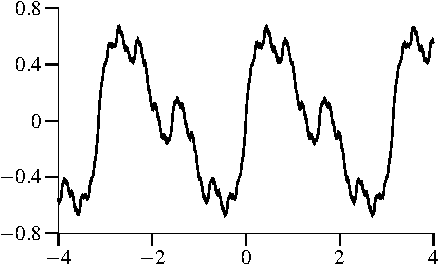
\includegraphics{figures/fourierserweier}
\caption{Plot of 
$\sum_{n=1}^\infty \frac{1}{2^n} \sin(2^n x)$.\label{fig:fourierserweier}}
\end{myfigureht}

\begin{exercise}
Given a $2\pi$-periodic function $f \colon \R \to \C$ Riemann integrable on
$[-\pi,\pi]$,
and $\epsilon > 0$.
Show that there exists a continuous $2\pi$-periodic function $g \colon \R
\to \C$ such that $\snorm{f-g}_2 < \epsilon$.
\end{exercise}

\begin{exercise}
Prove the Cauchy-Bunyakovsky-Schwarz inequality
for Riemann integrable functions:
\begin{equation*}
{\abs{\int_a^b f\widebar{g}}}^2
\leq
\left( \int_a^b \sabs{f}^2 \right)
\left( \int_a^b \sabs{g}^2 \right) .
\end{equation*}
\end{exercise}

\begin{exercise}
Prove the $L^2$ triangle inequality for
for Riemann integrable functions:
\begin{equation*}
\snorm{f+g}_2 \leq \snorm{f}_2 + \snorm{g}_2 .
\end{equation*}
\end{exercise}

